\documentclass[a4paper]{article}

% CJK support: prefer ctex, fallback to XeTeX native line breaking
\IfFileExists{ctex.sty}{
  \usepackage[fontset=fandol]{ctex}
}{
  % Fallback for minimal TeX installs (e.g. MacTeX Basic, TeX Live scheme-basic)
  % without ctex/xeCJK. Uses XeTeX's built-in CJK line breaking.
  \usepackage{fontspec}
  \XeTeXlinebreaklocale "zh"
  \XeTeXlinebreakskip = 0pt plus 1pt
  \IfFontExistsTF{Songti SC}{\setmainfont{Songti SC}}{%
    \IfFontExistsTF{Noto Serif CJK SC}{\setmainfont{Noto Serif CJK SC}}{}%
  }
  \IfFontExistsTF{Heiti SC}{\setsansfont{Heiti SC}}{%
    \IfFontExistsTF{Noto Sans CJK SC}{\setsansfont{Noto Sans CJK SC}}{}%
  }
}

% Basic packages
\usepackage{amsmath, amssymb}
\usepackage{graphicx}
\usepackage[margin=2.5cm]{geometry}
\emergencystretch=3em
\usepackage[most]{tcolorbox}
\usepackage{etoolbox}
\usepackage{listings}
\usepackage{hyperref}
\usepackage{booktabs}
\usepackage{array}
\usepackage{subcaption}
\usepackage{float}
\usepackage{tikz}
\IfFileExists{pgfplots.sty}{
    \usepackage{pgfplots}
    \pgfplotsset{compat=1.18}
}{}

% ===== Highlight boxes =====
\newtcolorbox{knowledgebox}[1]{
    enhanced, colback=blue!5!white, colframe=blue!75!black, colbacktitle=blue!75!black,
    coltitle=white, fonttitle=\bfseries, title={#1}, attach boxed title to top left={yshift=-2mm, xshift=2mm},
    boxrule=1pt, sharp corners
}

\newtcolorbox{importantbox}[1]{
    enhanced, colback=yellow!10!white, colframe=yellow!80!black, colbacktitle=yellow!80!black,
    coltitle=black, fonttitle=\bfseries, title={#1}, sharp corners
}

\newtcolorbox{warningbox}[1]{
    enhanced, colback=red!5!white, colframe=red!75!black, colbacktitle=red!75!black,
    coltitle=white, fonttitle=\bfseries, title={#1}, sharp corners
}

\newtcolorbox{practicebox}[1]{
    enhanced, colback=black!3!white, colframe=black!75, colbacktitle=black!75,
    coltitle=white, fonttitle=\bfseries, title={#1}, sharp corners
}

% ===== Code listings =====
\lstset{
    basicstyle=\ttfamily\small,
    keywordstyle=\color{blue},
    stringstyle=\color{red!60!black},
    commentstyle=\color{green!60!black},
    breaklines=true,
    frame=single,
    numbers=left,
    numberstyle=\tiny\color{gray},
    captionpos=b,
    extendedchars=false
}

% ===== Figure provenance and unit macros =====
% \vtag goes inside \caption{...}; \srcnote{MM:SS--MM:SS} follows the figure environment.
\newcommand{\vtag}{\protect\footnotemark}
\newcommand{\srcnote}[1]{\footnotetext{视频画面时间区间：#1。若为裁剪图，时间区间仍对应原视频画面。}}
% Units work in text and math mode; never hand-write $^\circ$ or \AA inside \mathrm.
\newcommand{\degC}{\ensuremath{^{\circ}\mathrm{C}}}
\newcommand{\um}{\ensuremath{\mu\mathrm{m}}}
\newcommand{\nm}{\ensuremath{\mathrm{nm}}}
\newcommand{\angstrom}{\ensuremath{\text{\AA}}}

% ===== Front-page metadata =====
% Fill these in when generating notes.
\newcommand{\notetitle}{版本控制与 Git}
\newcommand{\notesubtitle}{MIT Missing Semester 2026 · 第 5 讲：快照、提交图、对象与引用，以及分支、合并与远程协作}
\newcommand{\noteauthors}{根据 MIT Missing Semester 2026 课堂录像整理（Anish 主讲）}
\newcommand{\notedate}{2026年1月16日（课堂）}
\newcommand{\videochannel}{Missing Semester（YouTube）}
\newcommand{\videopublishdate}{2026年}
\newcommand{\videoduration}{1小时9分32秒}
\newcommand{\videourl}{https://www.youtube.com/watch?v=9K8lB61dl3Y}
\newcommand{\videocoverpath}{cover.jpg}

\setlength{\emergencystretch}{3em}
\begin{document}

% ===== Title page =====
\begin{titlepage}
\centering
{\Large 课程笔记\par}
\vspace{1.2cm}
{\huge\bfseries \notetitle\par}
\ifdefempty{\notesubtitle}{}{
\vspace{0.3cm}
{\large \notesubtitle\par}
}
\vspace{0.5cm}
{\large \noteauthors\par}
\vspace{0.3cm}
{\large \notedate\par}
\vspace{1.0cm}

\ifdefempty{\videocoverpath}{
{\small 请在生成笔记时填入视频封面图的本地路径。\par}
}{
\includegraphics[width=0.82\textwidth,height=0.40\textheight,keepaspectratio]{\videocoverpath}\par
}

\vfill
\begin{tcolorbox}[width=0.9\textwidth, colback=black!2!white, colframe=black!60, sharp corners]
\textbf{视频作者/频道}：\videochannel\par
\textbf{发布日期}：\videopublishdate\par
\textbf{视频时长}：\videoduration\par
\textbf{视频链接}：
\ifdefempty{\videourl}{
未填写
}{
\href{\videourl}{\nolinkurl{\videourl}}
}
\end{tcolorbox}
\end{titlepage}

\tableofcontents
\newpage

%% --- 正文内容开始 --- %%

\section{这一讲讲什么}

这一讲的主题是版本控制系统，特别是 Git，因为它是当今非常流行的版本控制系统。讲者 Anish 先解释什么是版本控制系统：它是一种软件，用来跟踪源代码，或者任何你想跟踪变化的文件和文件夹的变化。顾名思义，这些工具帮助你维护所编写软件的变更历史；此外，它们还便于协作。比如使用 GitHub 这样的开发平台时，你会用 Git 与这个服务、与在同一代码库上工作的其他开发者交互。

从逻辑上看，版本控制系统跟踪一个包含代码等文件的文件夹及其全部内容的变化，形成一系列快照，并保存一些元数据，比如每个快照是谁创建的，以及你想附加在修改上的消息，也许用来解释为什么做这些修改。

\subsection{为什么版本控制有用}

讲者说，即使不与别人协作，只是做一个习题或实验作业，版本控制也能让你查看项目的旧快照，基本上就是在你修改代码的过程中跟踪它；它还支持并行的开发分支：在同一个代码基础上做功能一，没做完时切换去做功能二，又发现一个 bug 想去修，这些都能在版本控制系统的帮助下完成，而不必把整个项目复制成一堆副本，那样很快就会一团糟。它也是做软件开发时与他人协作的标准工具。

现代版本控制系统还能回答许多原本很难回答的问题：这段代码或这个模块是谁写的？想找他聊聊。某一行代码最后是谁改的？什么时候改的？为什么改？甚至可以做一些花哨的事：假设你维护一个软件好几个月了，有一天发现它有个 bug，而一年前它还好好的，中间某个时候被引入了，版本控制系统能帮你找出是哪次修改引入的。

\section{为什么 Git 难学}

\subsection{Git 的名声}

\noindent\begin{minipage}{\textwidth}
\begin{figure}[H]
\centering
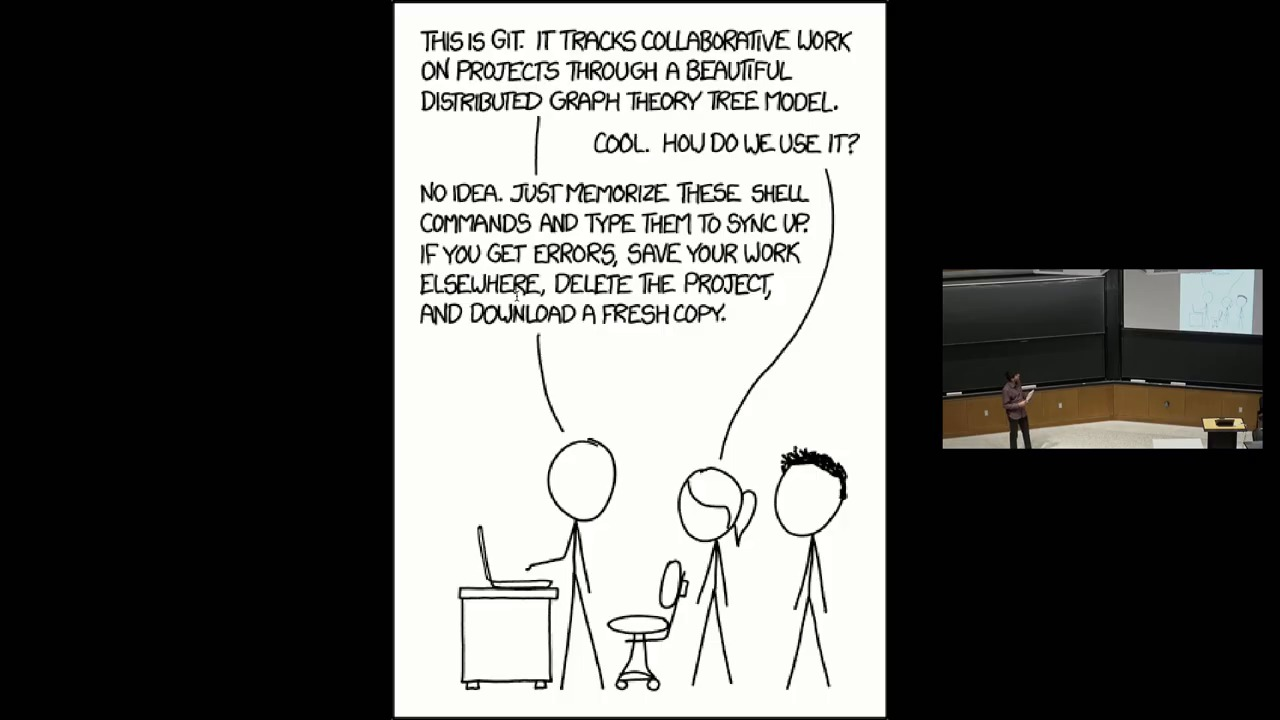
\includegraphics[width=0.92\textwidth]{figures/fig_01_xkcd.jpg}
\caption{xkcd 漫画：记住几条命令，出错就删掉项目重新下载一份\vtag}
\end{figure}
\srcnote{00:03:30--00:03:45}
\end{minipage}


讲者说，这一讲会讲版本控制背后的概念，特别是 Git，因为它是事实上的标准。不幸的是 Git 名声复杂。他读了屏幕上的 xkcd 漫画：“这是 Git。它用一个美丽的分布式图论树模型跟踪项目上的协作。”“酷，怎么用？”“不知道。记住这些 Shell 命令，输入它们来同步。出错了就把工作存到别处，删掉项目，重新下载一份。”讲者问谁这样做过，不少人举手，包括他自己，在学这些工具时他也这样干过。这一讲的目标是让大家不再是漫画里的那个人。

为什么会这样？讲者认为 Git 的界面，也就是你用来操作它的命令，是一种有漏洞的抽象（leaky abstraction）。如果自顶向下学 Git，从命令及其作用开始，而不理解底层思想，就容易产生很多困惑：你可以背下一堆命令，知道什么时候用，把它们大致当作魔法咒语；出了问题就删掉仓库重来。但这样显然没有有效地使用这个工具。Git 的界面也许不是最干净的，但它底层的思想可以被深刻理解。

\begin{importantbox}{自底向上学 Git}
因此这一讲采用自底向上的讲法：先讲底层思想和数据模型，再从高层讲命令行界面，并给出进一步学习、记住所需命令的指引。讲者认为这是学 Git 的正确方式，而网上大多数学习资源并不是这样讲的。
\end{importantbox}

\section{数据模型：快照与历史}

讲者说，不必担心那个“复杂的分布式图论树模型”，它其实很简单，而且能优雅地支持前面讲的那些功能：查看谁做了修改、跟踪变化、维护历史、支持不同的开发分支、与其他开发者协作。

\subsection{快照：blob 与 tree}

\noindent\begin{minipage}{\textwidth}
\begin{figure}[H]
\centering
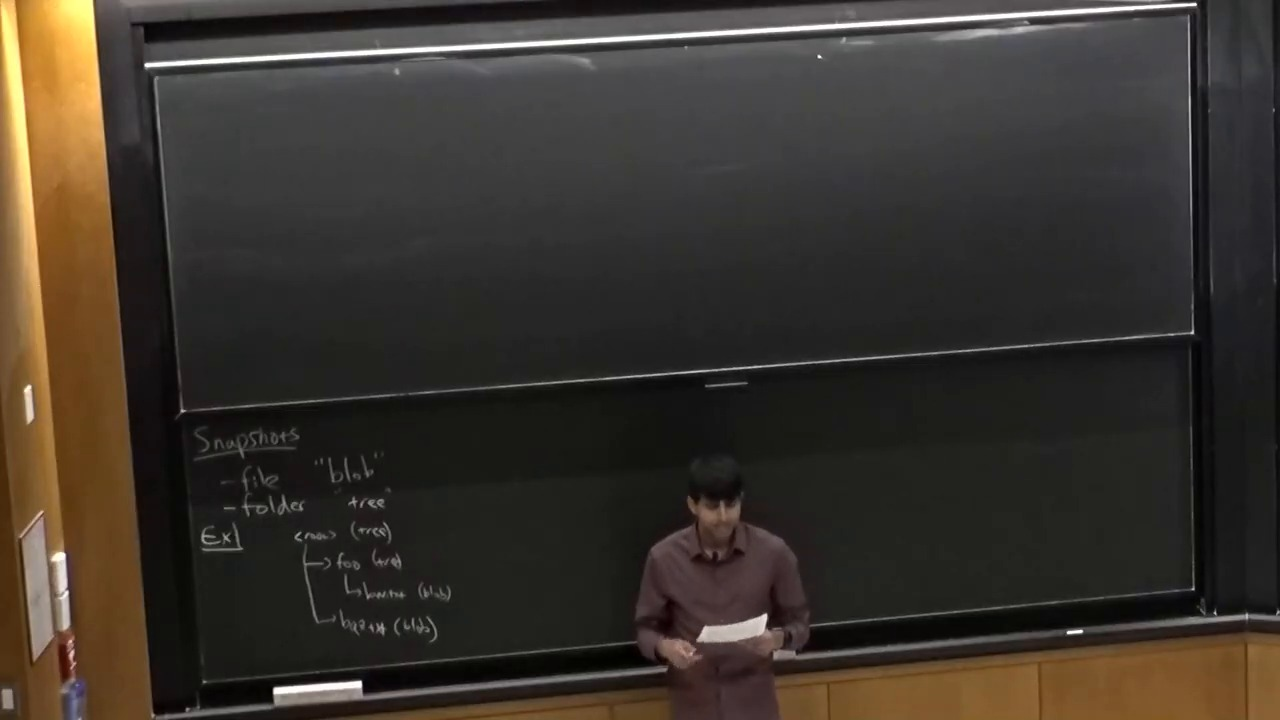
\includegraphics[width=0.92\textwidth]{figures/fig_02_snapshot_tree.jpg}
\caption{黑板上的快照示例：根 tree 下有子 tree foo 和文件 baz.txt\vtag}
\end{figure}
\srcnote{00:08:15--00:08:30}
\end{minipage}


数据模型的起点是快照。讲者用这个词指一个目录及其中一切内容的状态，也就是电脑上文件和文件夹的层次结构。Git 把历史中的某个时间点建模为文件和文件夹的集合，即快照。在 Git 术语中，文件叫 blob，文件夹叫 tree。一个快照的例子：快照的根目录是一个 tree；里面有另一个 tree，叫 foo；foo 里面有一个文件 bar.txt，是一个 blob；顶层 tree 里还有另一个文件 baz.txt。这样就刻画了一个文件夹及其中一切的状态。

\subsection{历史：快照的有向无环图}

\noindent\begin{minipage}{\textwidth}
\begin{figure}[H]
\centering
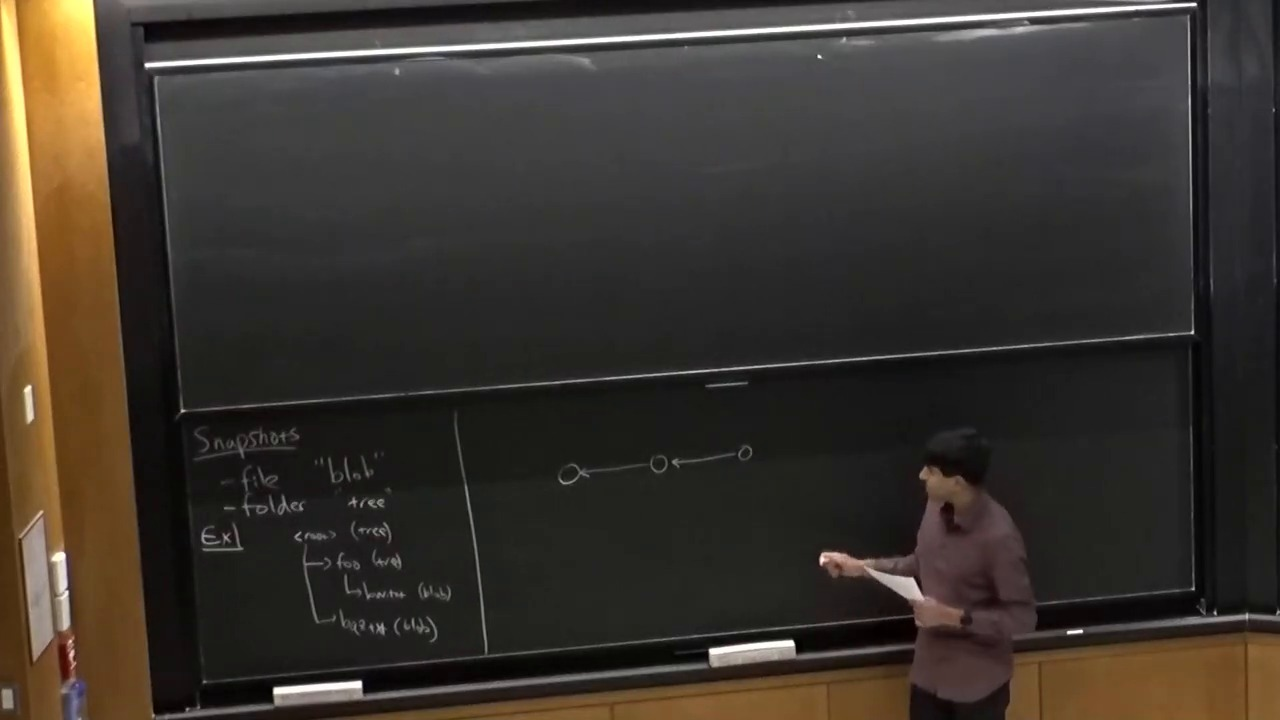
\includegraphics[width=0.92\textwidth]{figures/fig_03_history_dag.jpg}
\caption{每个快照指向它的父快照，从同一个快照分出两条开发线\vtag}
\end{figure}
\srcnote{00:09:30--00:09:45}
\end{minipage}


接下来，怎样把快照联系起来，维护历史？一种想法是简单存一个快照序列：版本一、版本二、版本三，看不同快照就能知道变化。出于一些原因，Git 不这样建模历史，而是稍微花哨一点：在 Git 中，历史是快照的有向无环图（directed acyclic graph，DAG）。讲者说没学过数据结构与算法也不要紧，这不复杂，意思只是每个快照指向一组父快照，即在它之前的那些。

比如从某个状态开始，修改代码，加了一个功能，得到一个新快照，它指回之前的快照；再修一个 bug，又得到一个新快照，指回前一个。假如此时既想实现一个功能，又想修一个 bug，可以基于同一个快照独立地做这两件事：从这里分出去修 bug，创建新快照；同时从同一个起点出发，推进功能的实现。

\noindent\begin{minipage}{\textwidth}
\begin{figure}[H]
\centering
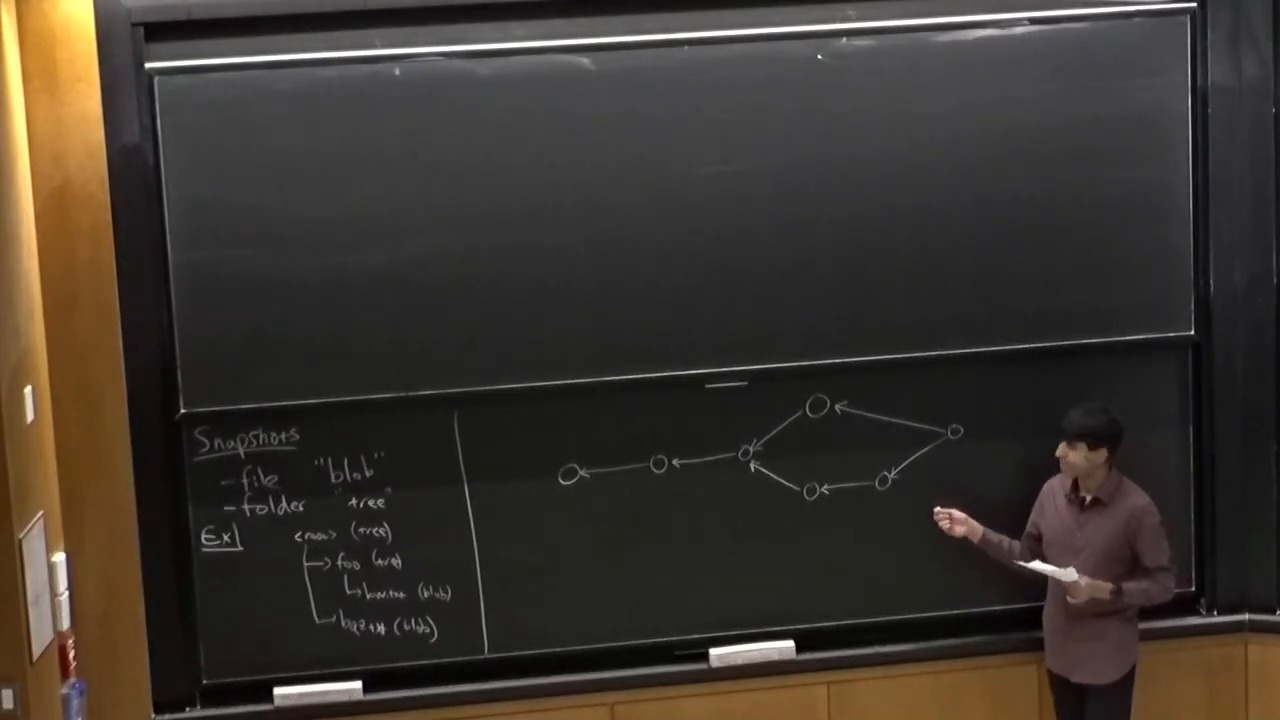
\includegraphics[width=0.92\textwidth]{figures/fig_04_merge_commit.jpg}
\caption{bug 修复分支和功能分支汇合成一个有两个父节点的合并提交\vtag}
\end{figure}
\srcnote{00:10:30--00:10:45}
\end{minipage}


到此为止展示的是分叉，也可能有一个快照有多个父节点：修 bug 的分支修好了，功能分支的功能也终于完成了，你想把两组修改合并成一个统一的代码库，于是创建一个包含两者修改的提交，它把两者都作为父节点，因为它是从两者派生出来的，这叫合并提交（merge commit）。这就是 Git 在逻辑上表示历史的方式：一堆通过父子关系联系起来的快照。

\begin{warningbox}{历史是不可变的}
讲者强调，这整个结构是不可变的数据结构：可以往上添加，创建一个新提交指向之前的提交，但不能修改其中已有的东西。就像现实中不能回到过去改变历史一样，Git 想如实记录发生过的历史，只能追加。对于各种错误，比如不小心引入了 bug、想撤销某个提交，有办法达到同样的效果，而不必真的去改动这个只追加的结构。
\end{warningbox}

\subsection{用伪代码描述}

\noindent\begin{minipage}{\textwidth}
\begin{figure}[H]
\centering
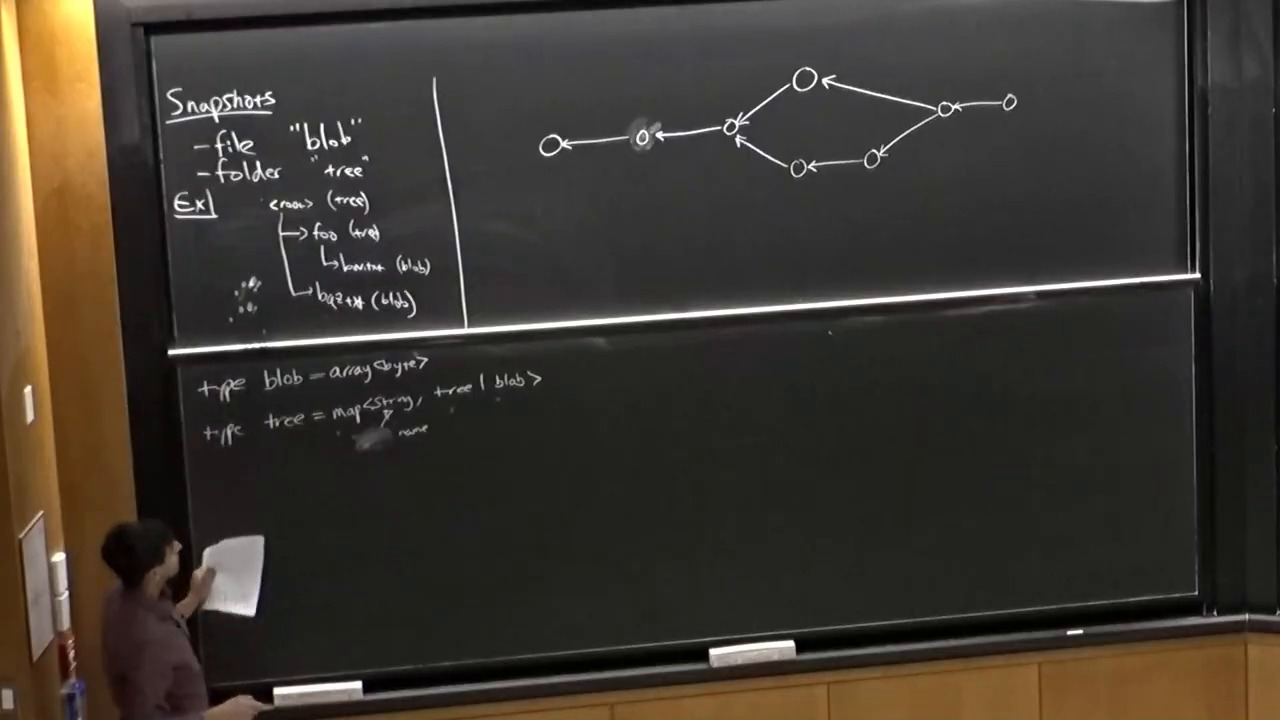
\includegraphics[width=0.92\textwidth]{figures/fig_05_pseudo_types.jpg}
\caption{黑板上的类型定义：blob 是字节数组，tree 是名字到 tree 或 blob 的映射\vtag}
\end{figure}
\srcnote{00:13:30--00:13:45}
\end{minipage}


讲者说，用更像代码的方式把这些概念写下来会很有启发，于是在黑板上写了一些类型定义。在 Git 里，文件（blob）是什么？就是一串数据，字节数组，电脑上的文件本来就是二进制数据。tree（目录）是什么？是把内容的名字映射到实际内容的数据结构：比如前面的顶层 tree 把 foo 映射到它里面的 tree，把 baz.txt 映射到里面的 blob。所以 tree 的元素可以是 tree 或 blob，用名字标识。

\noindent\begin{minipage}{\textwidth}
\begin{figure}[H]
\centering
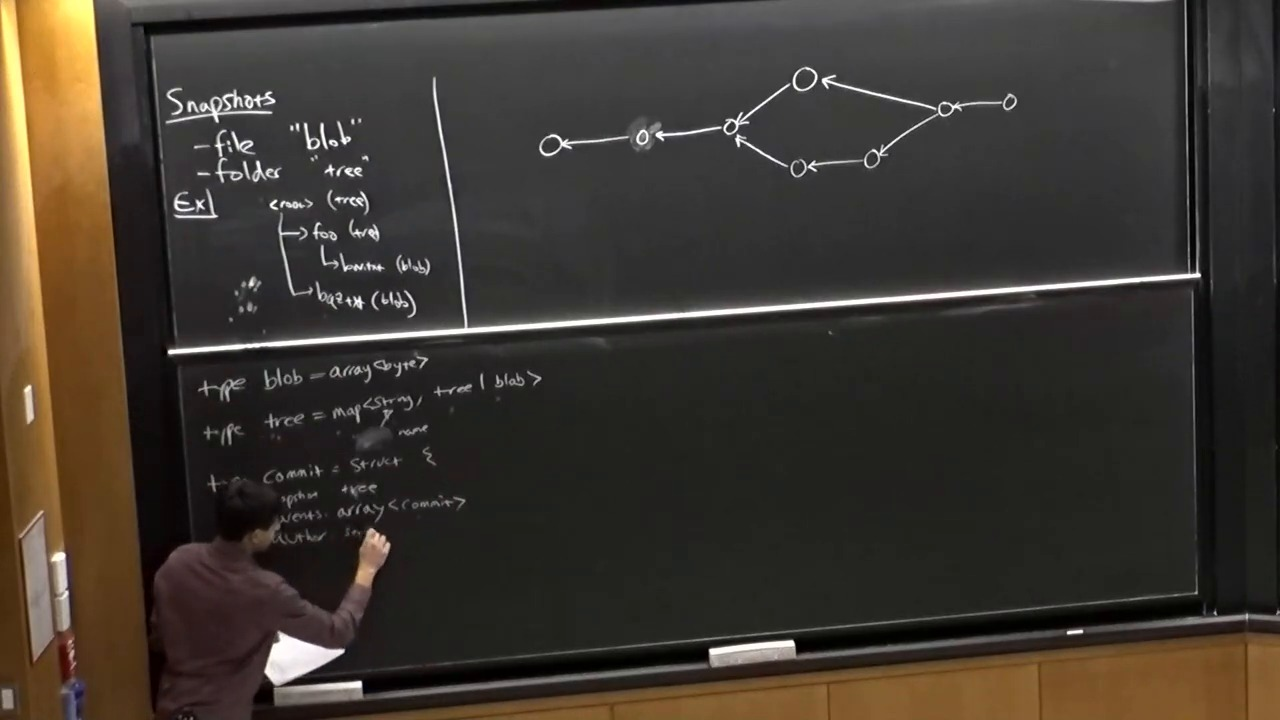
\includegraphics[width=0.92\textwidth]{figures/fig_06_commit_struct.jpg}
\caption{提交的定义：父提交列表、作者、提交信息和快照\vtag}
\end{figure}
\srcnote{00:15:00--00:15:15}
\end{minipage}


讲者澄清术语：说 blob 或 tree 时，指的是这个递归数据结构中的元素类型；说快照时（这不是标准的 Git 术语），指的是对应整个要跟踪历史的目录的顶层 tree；说提交（commit）时，指的是历史图中的节点。提交是包含几个元素的数据结构：一个快照，类型是 tree；一组父节点，是提交的列表；还有一些方便的东西，比如作者名，以及提交信息，可以写这次提交改了什么。

\begin{lstlisting}[language=Python]
// a file is a bunch of bytes
type blob = array<byte>

// a directory contains named files and directories
type tree = map<string, tree | blob>

// a commit has parents, metadata, and the top-level tree
type commit = struct {
    parents: array<commit>
    author: string
    message: string
    snapshot: tree
}
\end{lstlisting}

\section{数据模型：对象与引用}

\subsection{对象与内容寻址}

\noindent\begin{minipage}{\textwidth}
\begin{figure}[H]
\centering
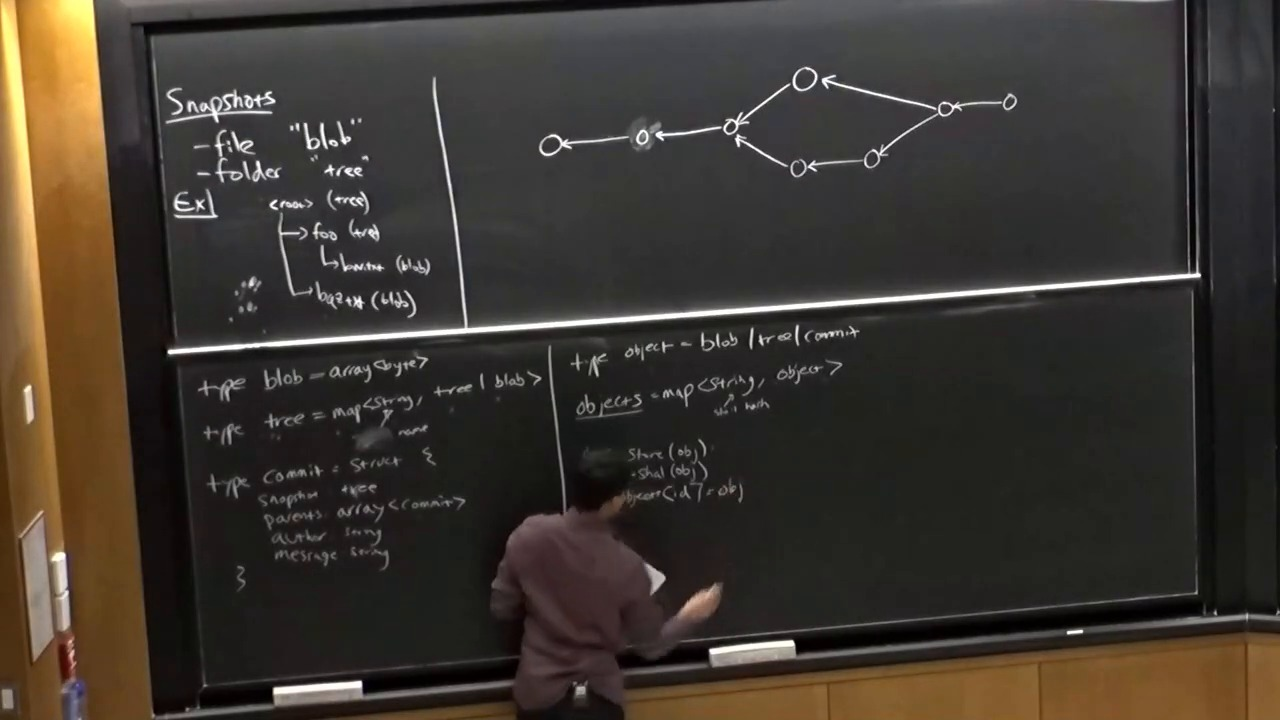
\includegraphics[width=0.92\textwidth]{figures/fig_07_object_store.jpg}
\caption{对象存储：objects 是从 SHA-1 哈希到对象的映射，store 先计算哈希再存入\vtag}
\end{figure}
\srcnote{00:17:00--00:17:15}
\end{minipage}


Git 引入了“对象”的概念，把 blob、tree 和 commit 统一起来：对象是 blob、tree 或 commit 之一。这样就能用统一的语言指代它们。Git 把数据存放在一个对象存储中，按内容的 SHA-1 哈希寻址（content-addressed）。也就是说，Git 用一个从 SHA-1 哈希到对象内容的映射来跟踪对象。存储对象时，先计算对象的哈希作为 ID，再把它放进这个映射；按 ID 加载时，直接从对象存储中按 ID 取出。

\begin{lstlisting}[language=Python]
type object = blob | tree | commit

objects = map<string, object>

def store(o):
    id = sha1(o)
    objects[id] = o

def load(id):
    return objects[id]
\end{lstlisting}

讲者补充了一个细节：在磁盘上的表示中，这些对象并不真的包含其他对象。不是说提交里包含之前的所有提交，或者 tree 里包含所有内容；它们存的是对其他对象的引用，可以把它们看作指针。比如上面例子中的顶层 tree，作为对象存储中的一个对象，内容有两个条目：foo 对应里面那个 tree 的哈希，相当于指向它的指针；baz.txt 对应那个 blob 的哈希。有同学问对象存储是什么，讲者说可以把它看作 Git 仓库里的一个全局变量，存放所有按 SHA-1 哈希标识的对象。

\noindent\begin{minipage}{\textwidth}
\begin{figure}[H]
\centering
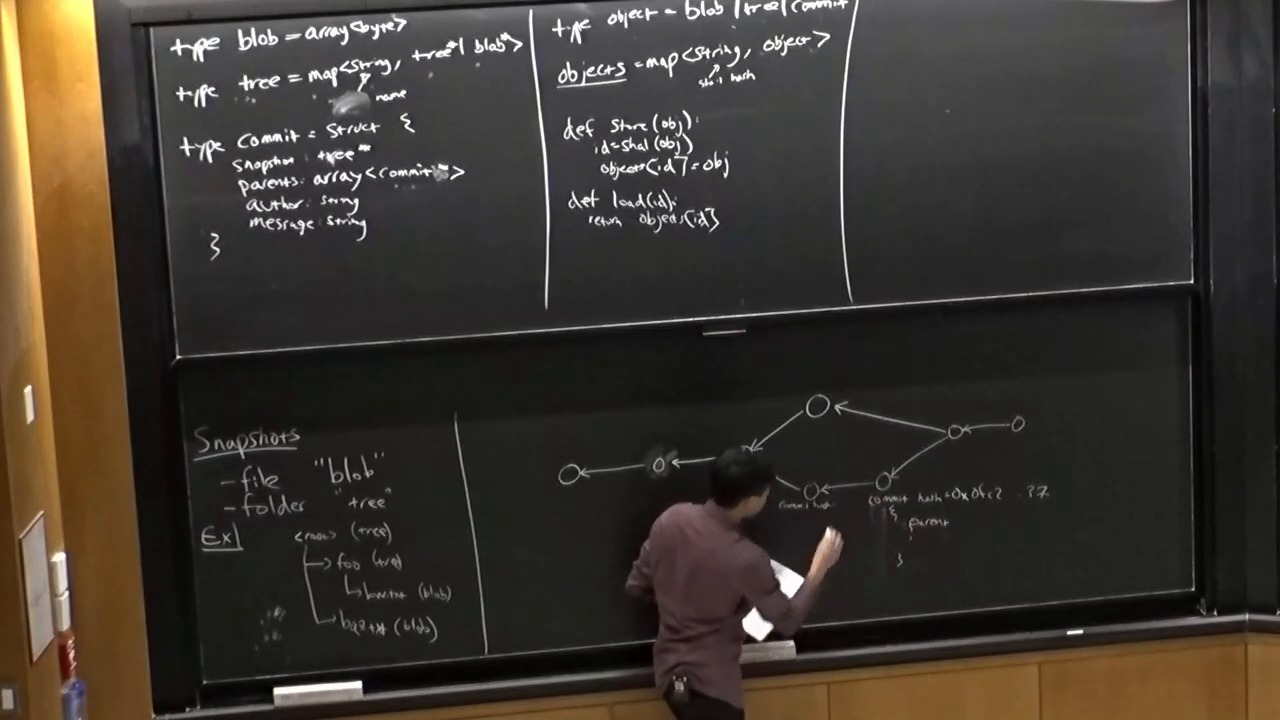
\includegraphics[width=0.92\textwidth]{figures/fig_08_hash_ids.jpg}
\caption{历史图中每个提交都标上了 40 位十六进制的哈希，父指针就是父提交的哈希\vtag}
\end{figure}
\srcnote{00:20:30--00:20:45}
\end{minipage}


在历史图上，每个提交也有一个哈希，Git 里通常写成 40 个字符长的十六进制字符串，比如 0fc2...37；它的内容中包括父指针，而哈希是对这些内容计算的。

\begin{knowledgebox}{什么是 SHA-1}
有同学问 SHA-1 是什么。讲者说它是一个哈希函数：输入任意长度的字节数组，输出 160 位的数据，可以把它看作把任意长度的数据随机但确定性地映射成固定长度的表示。他借用密码学中的随机预言机模型来解释：设想有一个全局登记处，第一次有人查询某个对象时，随机生成一个值记下来；以后任何人查同一个对象，都得到同一个值。总之，它以确定性的方式把任意大小的东西压缩成一个小的表示，看起来随机，碰撞很少：对两个不同的东西求哈希，得到相同输出的可能性非常小。讲义作者注：讲者口误说成了 160 字节，SHA-1 的输出是 160 位，即 20 字节，写成十六进制正好是 40 个字符。
\end{knowledgebox}

\subsection{引用}

\noindent\begin{minipage}{\textwidth}
\begin{figure}[H]
\centering
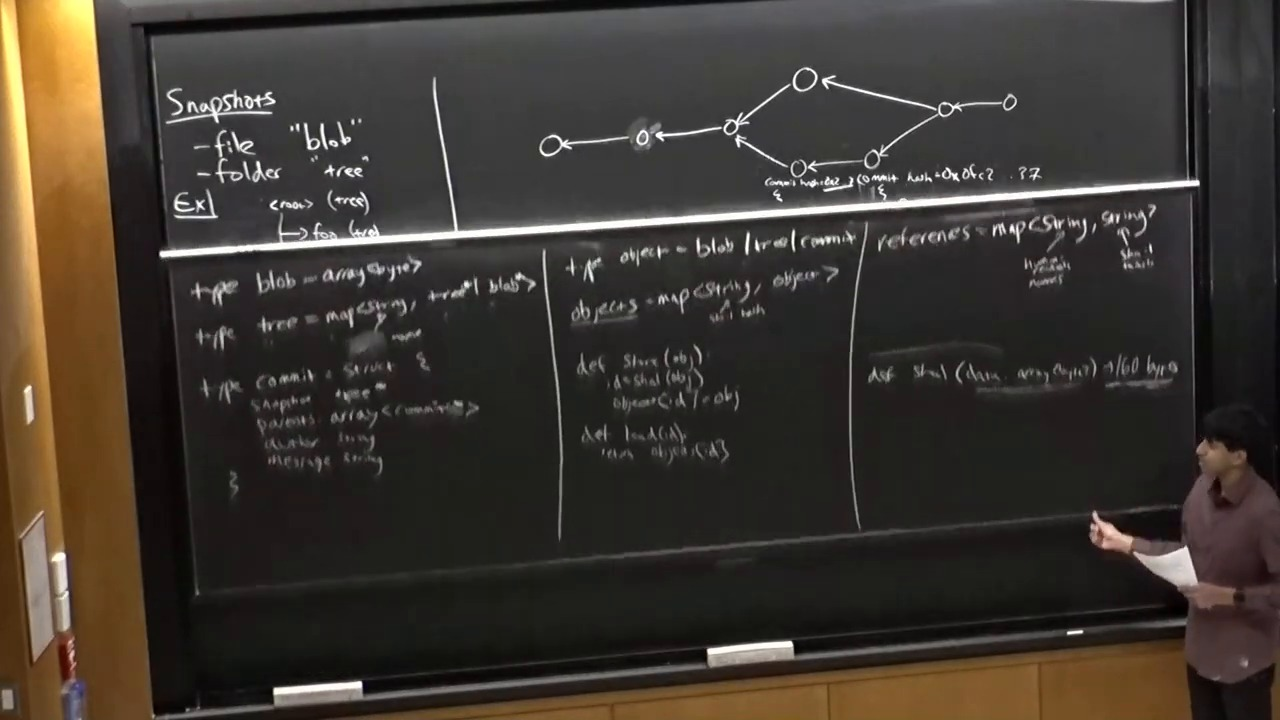
\includegraphics[width=0.92\textwidth]{figures/fig_09_references.jpg}
\caption{黑板上的引用：一个矩形标签指向某个提交，提交增加时标签随之前移\vtag}
\end{figure}
\srcnote{00:25:00--00:25:15}
\end{minipage}


现在我们有了用极不方便的 40 字符字符串命名东西的方式。Git 引入的下一个概念帮助命名：引用（references），把人类可读的名字映射到 SHA-1 哈希。讲者回顾：Git 历史是不可变的，对象存储里只往里放新东西，不删东西；而且由于哈希是对内容确定性计算的，同样的内容总得到同样的哈希。引用则不同：它可能是 Git 术语中的标签（tag）或分支（branch），指向提交图中的某个提交；因为引用映射是可变的，可以随着开发不断更新。黑板上的矩形就是指向某个提交的引用，开发时新增一个提交，就可以让引用指向新的提交。

有同学确认：提交和父子关系构成的历史是不可变的，而用来指代某些东西的名字，存放在引用数据结构中，是可变的。讲者说正是如此。

\begin{lstlisting}[language=Python]
references = map<string, string>

def update_reference(name, id):
    references[name] = id

def read_reference(name):
    return references[name]
\end{lstlisting}

\subsection{答疑：删除历史与合并冲突}

有同学问：如果在某处做了很糟糕的事，比如不小心提交了 API 密钥，而历史又是不可变的，怎么办？讲者说这是个复杂的话题。与人用 Git 协作时，实际上是你们共享一个不断增长的数据结构的不同切片：你做一些提交，另一个开发者做另一些，然后相互分享。如果已经分享出去才发现有 API 密钥，可以创建一份不包含它的新历史，于是得到整段历史的修改版本，\texttt{git rebase} 等命令可以做到这一点，讲义习题里有相关指引。另一种办法是：如果已经让那个 API 密钥失效（通常本来就应该这样做），就可以把它留在历史里，没什么大不了。对于其他类型的修改，比如想撤销某次提交的效果，可以创建一个新的提交来反转它，命令是 \texttt{git revert}。

又有同学问：分叉之后要合并，创建合并提交时 Git 怎么知道该怎样组合两边的内容？讲者说 Git 有许多启发式方法来智能地合并：比如在大型代码库中，一个提交改了一个文件，另一个提交改了另一个文件，合并它们很直接；但如果两边改了同一个文件的同一处，Git 就无法自动决定，这叫合并冲突（merge conflict）。文件中会出现冲突标记，标出 Git 不知如何处理的地方，\texttt{git mergetool} 等工具可以帮你解决。讲者说，只要做真实的软件开发、与人在同一个 Git 仓库上工作，迟早会遇到它。

\begin{warningbox}{泄露的密钥要先作废}
讲义作者提醒：一旦把密钥推送到远程仓库，就应假定它已经泄露，第一步是立即在服务商处吊销或轮换它；重写历史只能让它从今后的克隆中消失，无法收回已经被别人拉取的副本。
\end{warningbox}

\subsection{仓库就是对象加引用}

\noindent\begin{minipage}{\textwidth}
\begin{figure}[H]
\centering
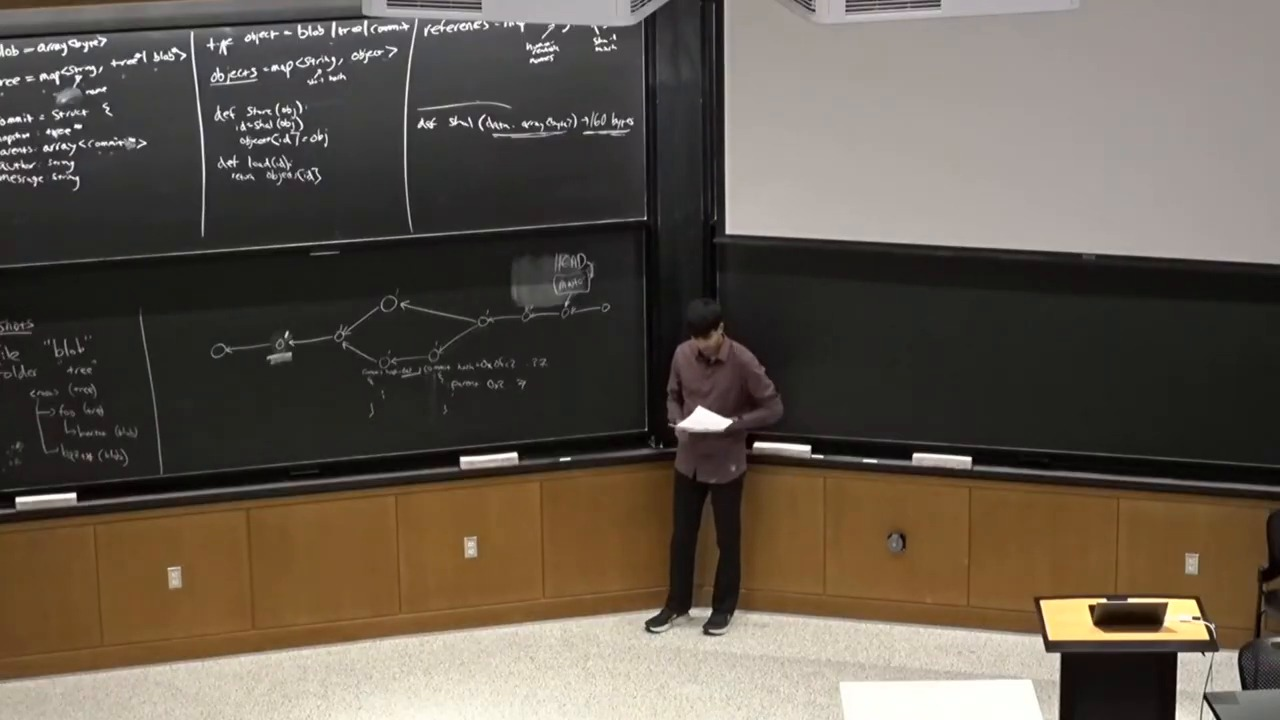
\includegraphics[width=0.92\textwidth]{figures/fig_10_full_model.jpg}
\caption{写满数据模型的黑板：blob、tree、commit、对象存储与引用\vtag}
\end{figure}
\srcnote{00:32:00--00:32:15}
\end{minipage}


讲者说，到这里已经讲完了 Git 数据模型的全部核心概念，终于可以定义什么是 Git 仓库：就是对象和引用的集合，仅此而已。就数据结构而言这些都是非常简单的概念，Git 核心有一些相当美的思想。在磁盘上，Git 为仓库存储的大致就是对象和引用。

有同学问 GitHub 是什么。讲者说 Git 是一个自由开源的分布式版本控制工具，GitHub 是一个提供 Git 仓库托管的软件即服务（SaaS）提供商，是人们托管开源软件、与他人协作的热门地方。比如作为学生，教授可能把实验作业放在一个 Git 仓库里，你克隆下来做作业；教授更新了作业，你可以直接拉取更新，而不必重新下载压缩包、解压、把你的改动复制过去或手动合并。GitHub 不是唯一的 Git 托管服务；而且某种意义上两者毫无关系：一个是现在归微软所有的公司，一个是开源软件。

\subsection{暂存区}

讲者最后介绍暂存区（staging area）。一种设计版本控制系统的方式是：跟踪电脑上的某个文件夹，提交命令就把它当前的样子“拍一张照”，作为新快照，有些版本控制系统就是这样工作的。Git 不同，它有一个暂存区，让你精确描述下一个快照包含什么：比如你写了一个功能，顺手加了一堆调试用的打印语句，又修了一个 bug，你可以只把功能和 bug 修复放进快照，而不包括那些打印语句，甚至可以把它们分成两个提交。他说会在接下来的演示中结合其他 Git 命令展示暂存区。

\begin{knowledgebox}{暂存区相关命令}
讲义作者补充：\texttt{git add 文件} 把文件的当前内容放入暂存区；\texttt{git add -p} 可以逐块挑选要暂存的修改，正好用于“只提交功能和修复、不提交调试打印”的场景；\texttt{git diff} 显示尚未暂存的修改，\texttt{git diff -{}-cached} 显示已暂存、将进入下一个提交的修改；\texttt{git restore -{}-staged 文件} 把文件移出暂存区。
\end{knowledgebox}

\begin{importantbox}{数据模型小结}
blob 是文件内容，tree 是目录，commit 指向一个顶层 tree 和若干父提交；三者统称对象，按内容的 SHA-1 哈希存放在只追加的对象存储中；引用（分支、标签）是指向提交的可变名字。理解了这些，几乎所有 Git 命令都可以理解为对对象图和引用的操作。
\end{importantbox}

\section{Git 命令行基础}

讲者做了个小调查：谁用过 Git？不少人举手。是想听基础，比如 \texttt{git init}、\texttt{git add}、\texttt{git branch}、\texttt{git merge} 并联系数据模型，还是远程仓库等中级内容，或者更花哨的东西？结果大致三等分。他说一定要讲完的是基础：如果理解了所有基础，能熟练使用远程仓库，那么对于更花哨的功能，只需要有人告诉你“这个东西存在”，你就可以自己去弄明白。

\subsection{git help 与 git init}

\noindent\begin{minipage}{\textwidth}
\begin{figure}[H]
\centering
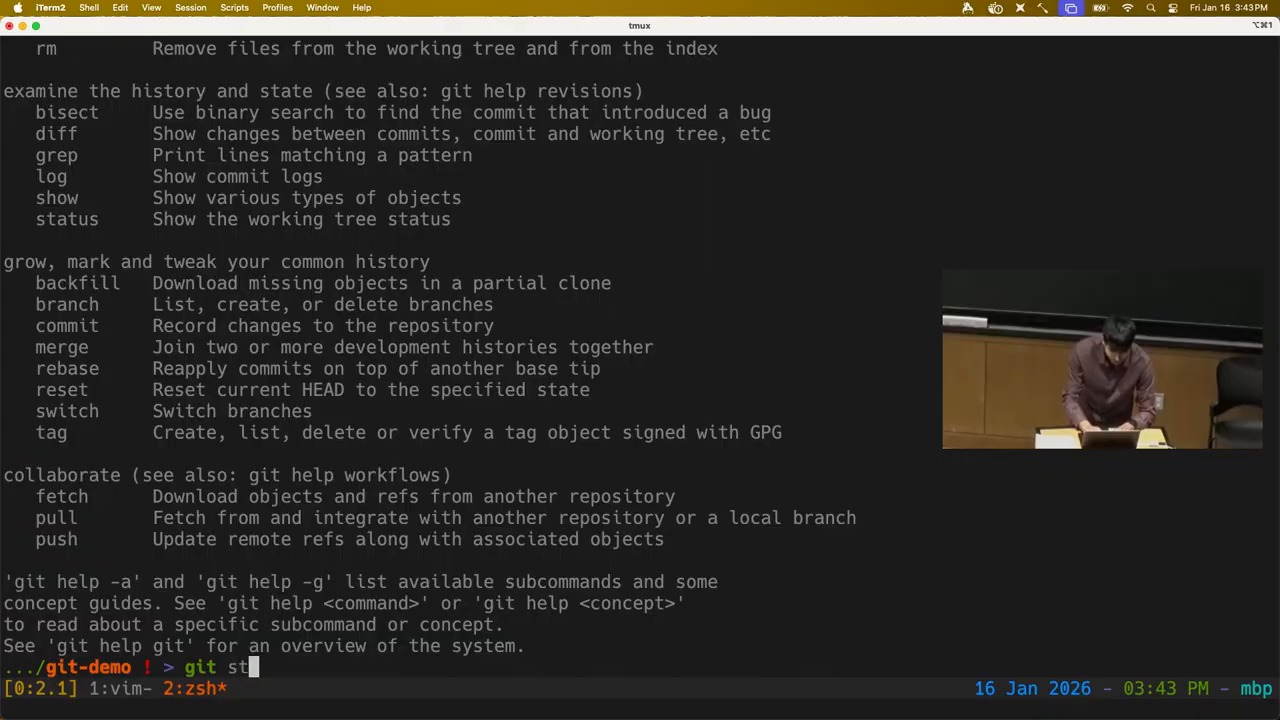
\includegraphics[width=0.92\textwidth]{figures/fig_11_git_help.jpg}
\caption{git help 列出常用子命令，每个子命令都有对应的手册页\vtag}
\end{figure}
\srcnote{00:38:00--00:38:15}
\end{minipage}


讲者说一个有用的命令是 \texttt{git help}。Git 的所有命令、所有功能都实现为 \texttt{git} 下的子命令，比如 \texttt{git status}、\texttt{git init}、\texttt{git commit}，可以通过 \texttt{git help} 获取子命令的帮助，它只是打开对应命令的手册页，第一讲讲过手册页，比如 \texttt{git help help}。

\noindent\begin{minipage}{\textwidth}
\begin{figure}[H]
\centering
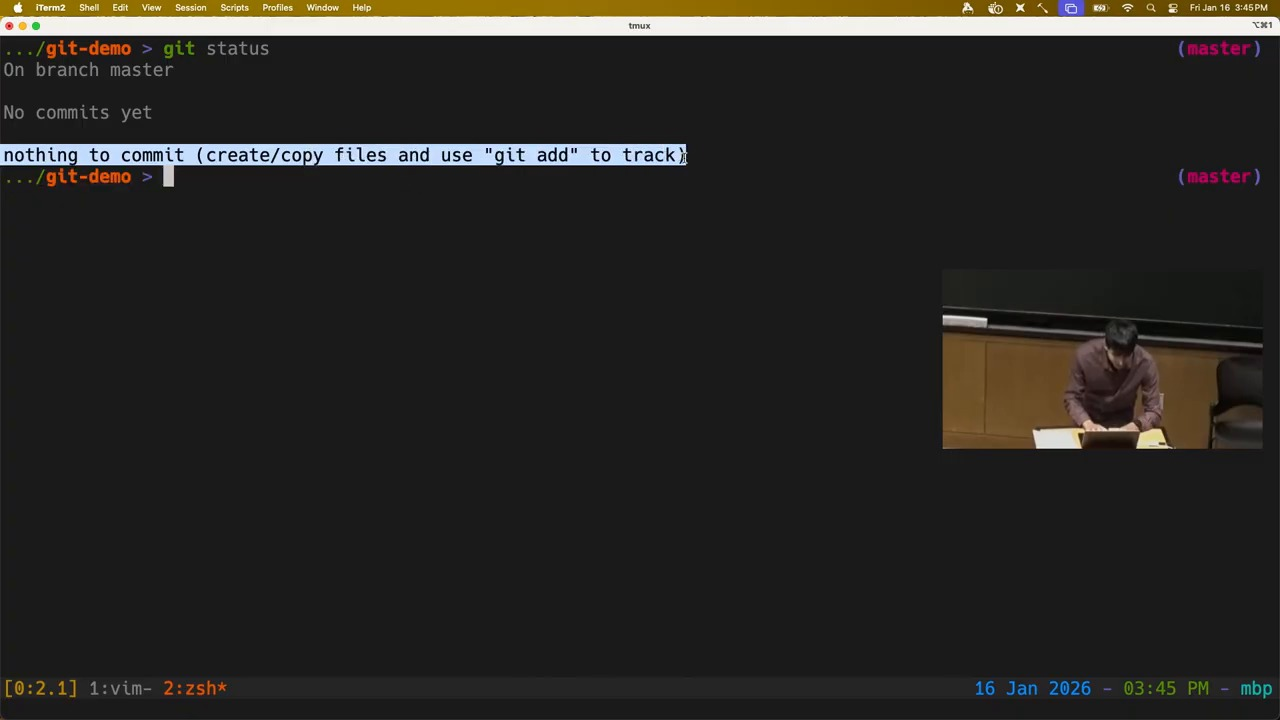
\includegraphics[width=0.92\textwidth]{figures/fig_12_git_status.jpg}
\caption{git init 后 git status 显示还没有任何提交，接着出现未跟踪的 nato.txt\vtag}
\end{figure}
\srcnote{00:39:30--00:39:45}
\end{minipage}


他用 \texttt{git init} 创建一个新仓库，它会创建一个隐藏的 \texttt{.git} 目录，用 \texttt{ls .git} 能看到 objects 和 refs 文件夹，分别存放对象存储（磁盘上的数据结构）和引用；想看底层细节可以自己创建仓库去翻看。\texttt{git status} 告诉你当前的情况：在 master 分支上，还没有提交。

有同学问：既然目录名是固定的，一个目录是不是只能有一个仓库？讲者说是的（带星号），他写软件这么多年，几乎没遇到过想把多个仓库放在同一目录的情况，非要这样也有办法；通常的做法是为每个仓库建单独的文件夹，比如很多人有一个 src 目录，里面每个项目一个子目录。

然后他写了一个文本文件 \texttt{nato.txt}，里面是北约音标字母（alpha、bravo、charlie……）。\texttt{git status} 显示有未跟踪的文件：Git 告诉你这个文件不在上一个快照里（这里还没有快照），只是提醒你它未被跟踪。

\subsection{add、commit 与 log}

\noindent\begin{minipage}{\textwidth}
\begin{figure}[H]
\centering
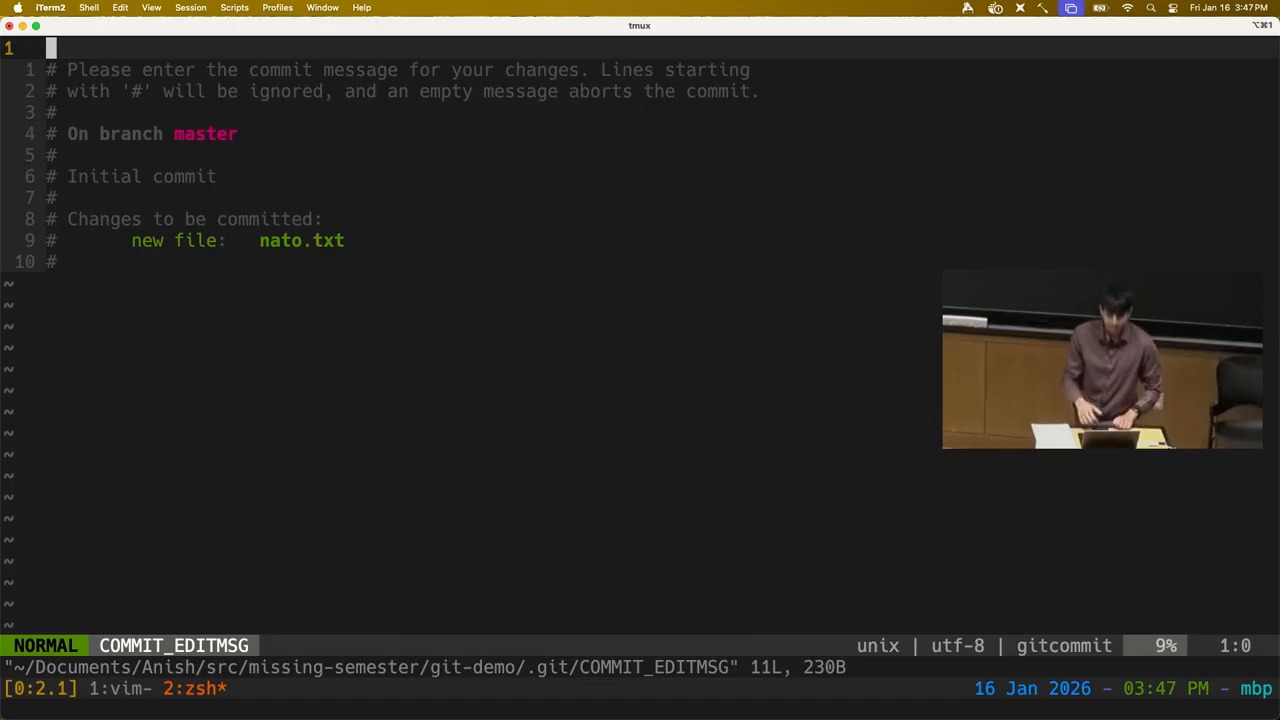
\includegraphics[width=0.92\textwidth]{figures/fig_13_commit_editor.jpg}
\caption{git commit 打开编辑器，在其中写下提交信息 Initial commit\vtag}
\end{figure}
\srcnote{00:42:00--00:42:15}
\end{minipage}


用 \texttt{git add nato.txt} 把文件放进暂存区，再用 \texttt{git commit} 创建新提交。它会打开一个编辑器，Git 会为提交附带一些元数据，包括提交信息，你应该写好的提交信息，这里就叫“Initial commit”。保存文件后，Git 读取其内容，创建一个名为 Initial commit 的提交。讲者说今天不讲怎样写好提交信息，讲义里有链接。

\texttt{git log} 显示历史的扁平视图，大致是把历史线性化后按顺序打印，它有一些选项，比如 \texttt{-{}-graph} 显示图形，只有一个提交时看不出什么，后面会看到更好看的图。

\begin{lstlisting}[language=bash]
git init
git status
git add nato.txt
git commit
git log --all --graph --decorate
\end{lstlisting}

\subsection{用 cat-file 查看对象}

\noindent\begin{minipage}{\textwidth}
\begin{figure}[H]
\centering
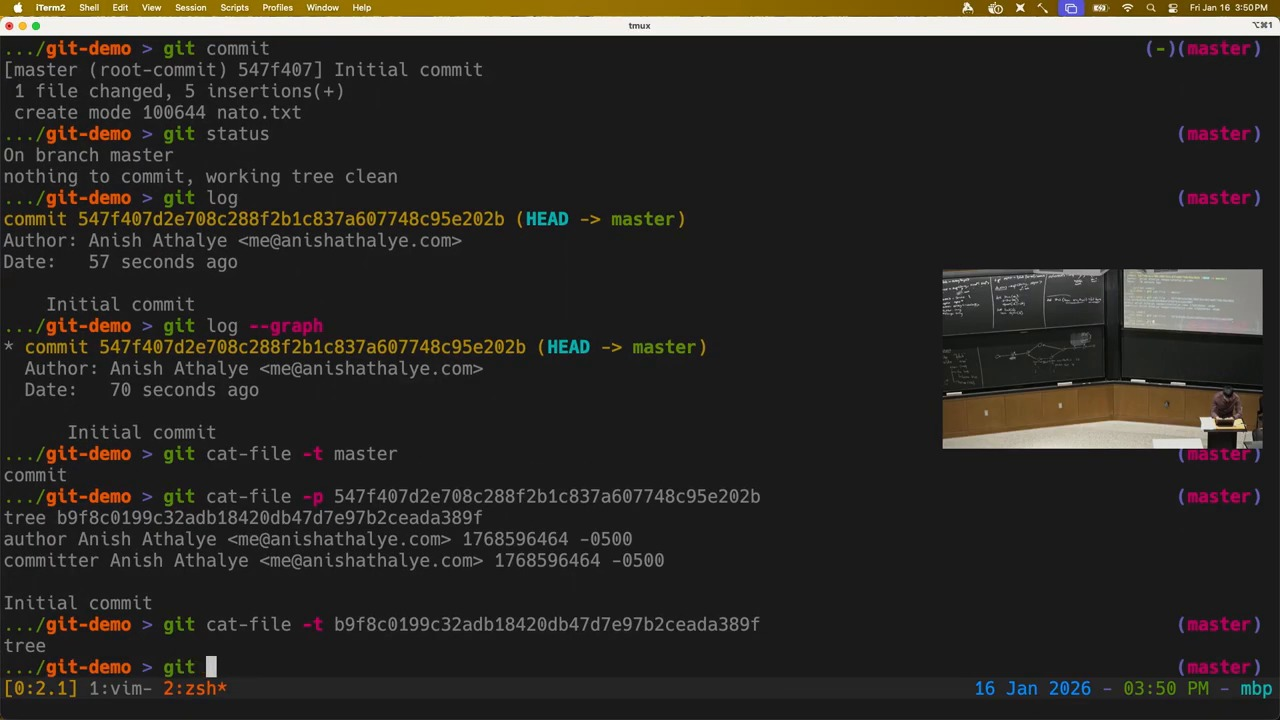
\includegraphics[width=0.92\textwidth]{figures/fig_14_cat_file.jpg}
\caption{git cat-file -p 依次打印提交、tree 和 blob 的内容\vtag}
\end{figure}
\srcnote{00:44:30--00:44:45}
\end{minipage}


为了联系数据模型，讲者用 \texttt{git cat-file} 查看底层数据。\texttt{git cat-file -p} 加上提交的哈希（Git 中所有对象都由对象哈希标识），就看到这个提交对应的数据：一个指向 tree 的指针，即这个快照的内容，一些元数据和提交信息；没有父节点，因为这是第一个提交。再对 tree 的哈希执行同样的命令，看到它包含一个条目 \texttt{nato.txt} 及其 blob 哈希；再对 blob 执行，就看到快照中这个文件的内容，这里和工作目录中的 \texttt{nato.txt} 相同。讲者说这就是把 Git 命令与底层数据模型联系起来的方式。

\begin{practicebox}{亲手走一遍对象图}
讲义作者整理：新建一个仓库并提交一个文件，然后用 \texttt{git cat-file -p HEAD} 查看提交，复制其中 tree 的哈希继续 \texttt{cat-file}，再复制 blob 的哈希查看文件内容；最后用 \texttt{git cat-file -t} 查看每个哈希对应的对象类型，并在 \texttt{.git/objects} 目录中找到这些对象对应的文件。
\end{practicebox}

\section{分支与合并}

\subsection{分支只是指针}

\noindent\begin{minipage}{\textwidth}
\begin{figure}[H]
\centering
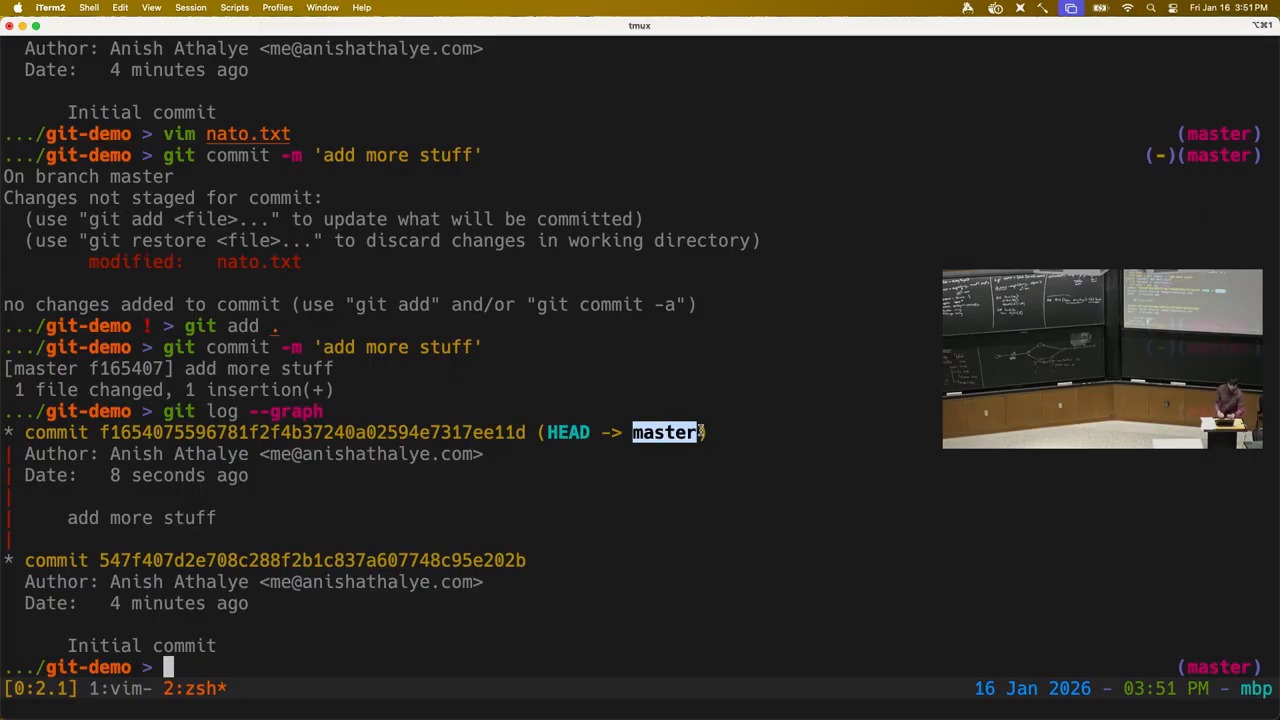
\includegraphics[width=0.92\textwidth]{figures/fig_15_branch_commit.jpg}
\caption{新提交 add more stuff 之后，master 引用随之前移到新提交\vtag}
\end{figure}
\srcnote{00:46:00--00:46:15}
\end{minipage}


有同学问分支是什么。讲者说分支是一种可以“附着”上去的特殊引用，你提交时它会跟着移动。\texttt{git log} 里只有一个提交，master 分支指向它。他往文件里加了一行文本并提交，于是有了原来的 Initial commit 和新提交，master 更新了：\texttt{git status} 说他在 master 分支上，\texttt{git commit} 就替他更新了这个引用。讲者说，前面讲可以把一切看作对底层数据模型的操作，但通常我们不做原子级的修改，Git 会把多个步骤组合成一条高层命令：\texttt{git commit} 创建 blob 和 tree 对象、创建提交对象，并更新当前分支。

有同学指出，直觉上可能以为分支指的是一整条谱系，但在 Git 中分支实际上只是一个指向提交的指针。讲者说完全正确：有些版本控制系统的分支概念不同，更接近跟踪谱系的直觉，但 Git 不是；分支只是指向提交的指针，可以随意移动。

\noindent\begin{minipage}{\textwidth}
\begin{figure}[H]
\centering
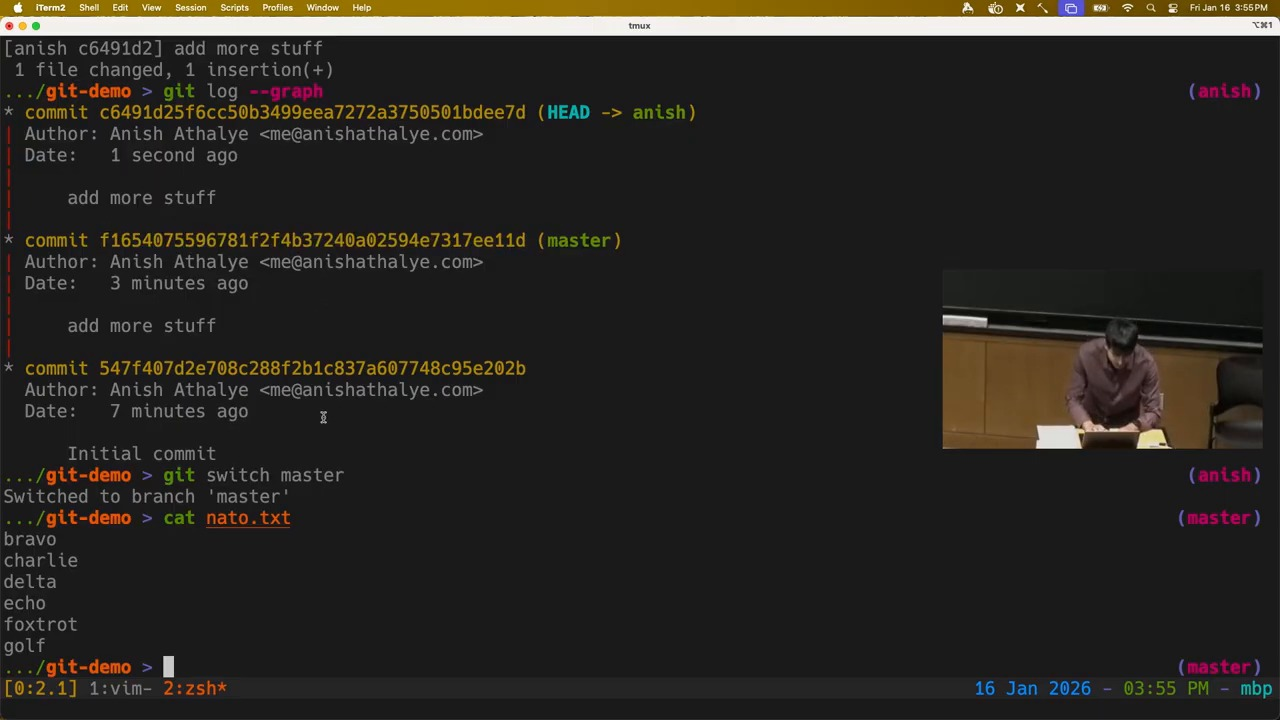
\includegraphics[width=0.92\textwidth]{figures/fig_16_switch_master.jpg}
\caption{git switch master 切回去后，工作目录里的 hotel 一行随之消失\vtag}
\end{figure}
\srcnote{00:49:30--00:49:45}
\end{minipage}


又有同学问 master 是否总是自动更新到最新的提交。讲者说不是。master 是（或者说曾经是）新建 Git 仓库时默认分支的名字；所有分支都这样工作：如果你附着在某个分支上并提交，那个分支就会更新。他用 \texttt{git branch anish} 在当前位置创建一个新分支，\texttt{git switch anish} 切过去，加了一行 hotel 并提交，anish 前移了，master 留在原地。再 \texttt{git switch master}，这会改变工作目录的内容：\texttt{cat nato.txt} 发现 hotel 不见了，因为回到了之前的快照。

\subsection{合并}

\noindent\begin{minipage}{\textwidth}
\begin{figure}[H]
\centering
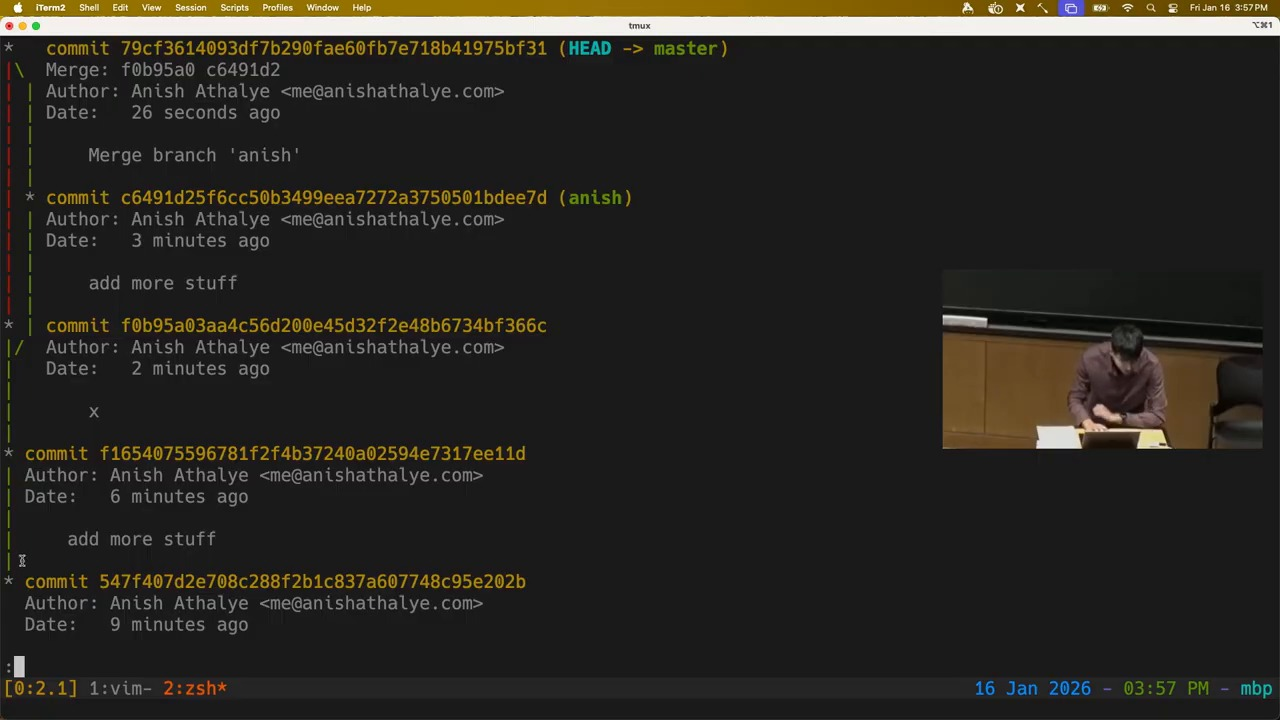
\includegraphics[width=0.92\textwidth]{figures/fig_17_merge_graph.jpg}
\caption{git log --graph 显示 anish 与 master 两条线汇合成合并提交\vtag}
\end{figure}
\srcnote{00:51:30--00:51:45}
\end{minipage}


在 master 上，他在文件顶部加了一行 alpha 并提交。新提交让 master 更新了，它的父节点是那个既没有 hotel 也没有 alpha 的提交，于是历史分叉了。讲者提到，\texttt{git log} 默认只显示从当前分支可达的历史，加上 \texttt{-{}-all} 才显示从所有分支可达的内容。

然后 \texttt{git merge anish}，它打开编辑器让你确认合并提交的信息，保存退出后显示 auto-merging nato.txt。因为一个修改在顶部加了 alpha，另一个在底部加了 hotel，中间内容相同，差异与合并算法足够聪明，知道应该把两者结合起来，所以没有合并冲突。再看历史，就能看到前几个提交、两条分叉，以及有两个父节点的合并提交。

\noindent\begin{minipage}{\textwidth}
\begin{figure}[H]
\centering
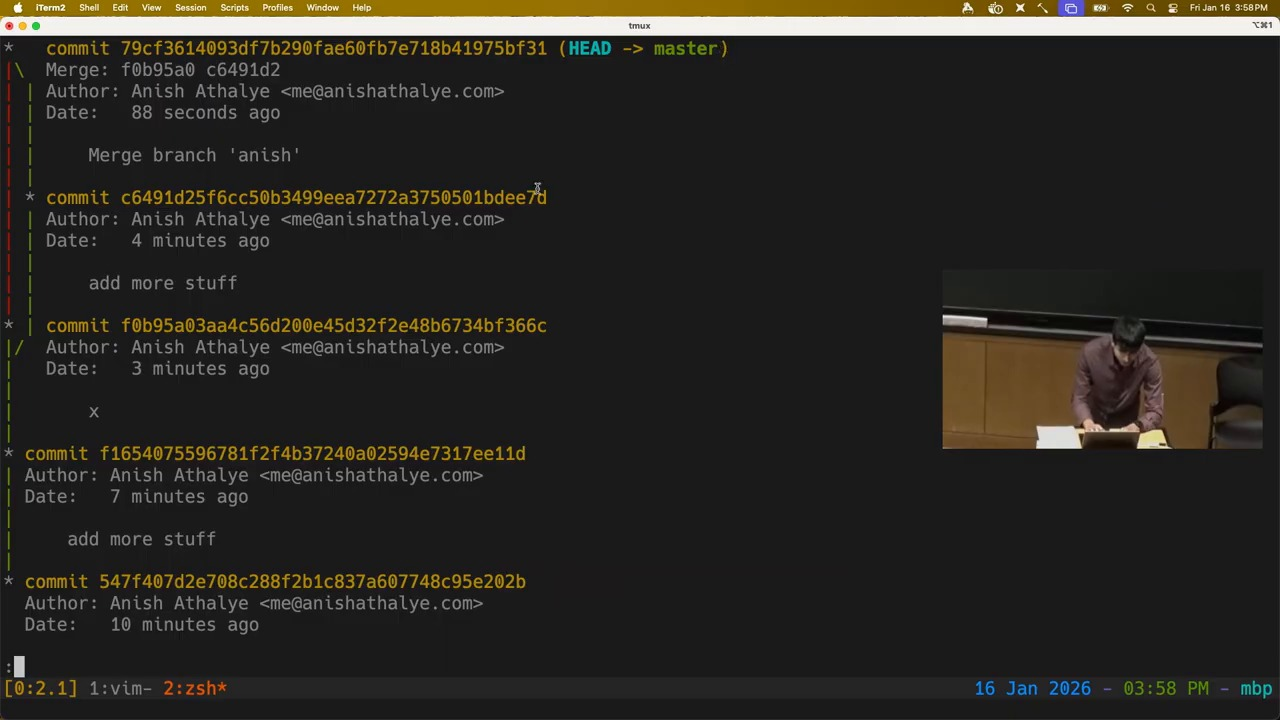
\includegraphics[width=0.92\textwidth]{figures/fig_18_branch_delete.jpg}
\caption{合并后用 git branch -d anish 删除已不再需要的分支名\vtag}
\end{figure}
\srcnote{00:52:30--00:52:45}
\end{minipage}


由于 master 已经包含了全部历史，包括 anish 上的修改，就不再需要这个名字了，可以 \texttt{git branch -d anish} 删除它。\texttt{git branch} 列出所有分支，当前所在的分支前面有绿色星号。讲者总结：分支只是提交的名字，或者说 SHA-1 哈希的名字；提交不可变，分支可变。

\begin{lstlisting}[language=bash]
git branch anish
git switch anish
git commit -am "add hotel"
git switch master
git commit -am "add alpha"
git merge anish
git branch -d anish
\end{lstlisting}

\noindent\begin{minipage}{\textwidth}
\begin{figure}[H]
\centering
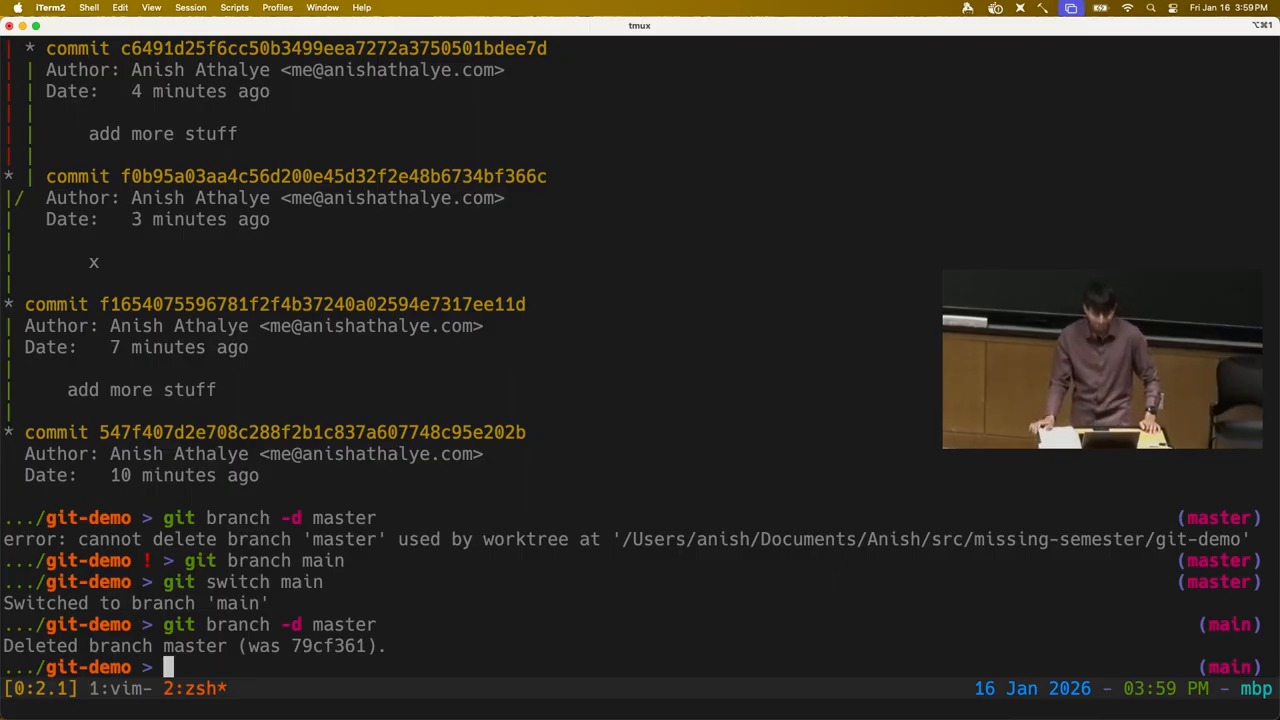
\includegraphics[width=0.92\textwidth]{figures/fig_19_rename_main.jpg}
\caption{删除当前所在的 master 失败，于是先建 main 并切换，再删除 master\vtag}
\end{figure}
\srcnote{00:54:00--00:54:15}
\end{minipage}


有同学问能否反过来把 master 合并进 anish。讲者说当然可以，master 没什么特别的，只是一个名字。又有同学问能否删除 master：讲者现场尝试，Git 拒绝了，因为 master 正在使用，HEAD 指向 master，表示当前检出的是它。于是他先 \texttt{git branch main}、\texttt{git switch main}，再删除 master，此后仓库的主分支就叫 main。

\begin{knowledgebox}{HEAD 是什么}
讲义作者补充：HEAD 是一个特殊的引用，表示“当前所在的位置”。通常它指向一个分支（例如 \texttt{HEAD -> main}），提交时被更新的是那个分支；直接检出某个提交时，HEAD 直接指向提交本身，就是后面要讲的分离 HEAD 状态。
\end{knowledgebox}

\subsection{reflog 与垃圾回收}

有同学问：误删了分支还能找回来吗？讲者说这是相当高级的 Git，如果一切都做对了，你永远不需要它，但有一个工具叫 \texttt{git reflog}。Git 维护一些额外的状态，包括引用的历史：引用是可变的，所以记录它们发生过什么往往很有用，比如一个分支从指向一个东西变成指向另一个东西。如果创建了一个提交又删掉了分支，可以在 reflog 里找到这个提交，它仍然在对象存储中。但对象存储里不被任何引用可达的“孤儿”对象，Git 会自动进行垃圾回收；所以如果用了一年之后才想起来，可能就找不回来了。

\noindent\begin{minipage}{\textwidth}
\begin{figure}[H]
\centering
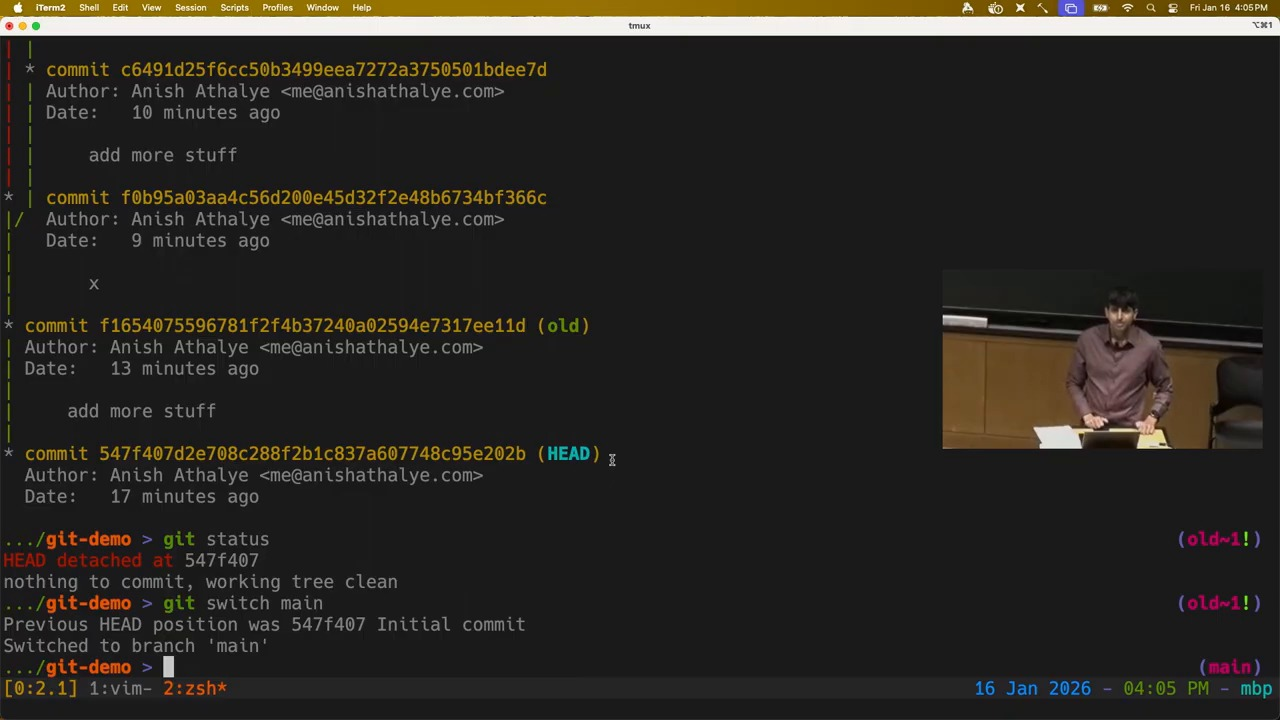
\includegraphics[width=0.92\textwidth]{figures/fig_20_detached.jpg}
\caption{git checkout 到旧提交后进入分离 HEAD 状态，git status 提示没有当前分支\vtag}
\end{figure}
\srcnote{00:59:30--00:59:45}
\end{minipage}


讲者接着演示了 \texttt{git checkout}：想把工作目录的内容改成某个旧提交，可以 \texttt{git checkout} 加那个提交（他先用 \texttt{git branch old} 给它起了个名字）。这会进入所谓的分离 HEAD（detached HEAD）状态，意思是当前没有活动分支；这时提交新内容，就不再有一个随你前进的具名分支。所以一般不会长时间停留在分离 HEAD 状态，通常你都在某个分支上修改代码。在这个状态下做了一个提交，再切回 main 时，Git 会警告：你留下了一个提交，它没有连接到任何分支。它暂时还在对象存储中，但因为没有分支指向它或它的后继，最终会被垃圾回收。

有同学在课后问：能不能用这时打印出的提交哈希创建新分支？讲者说可以，\texttt{git branch 新分支名 哈希} 就会在那个位置创建分支。

\subsection{分支的使用约定}

有同学问是否约定俗成地有 main 或 master 分支。讲者说是的，通常最新版本的代码放在 main 或 master 上（过去默认叫 master，现在一般叫 main）。常见做法是创建所谓的功能分支（feature branch），在上面修改，再合并回 main。还有更复杂的工作流：比如维护一个网站，有真实用户使用的生产版本，还有用于测试的预发布（staging）版本，于是可能有生产用的 main 分支和预发布用的 staging 分支，等等。

\begin{warningbox}{switch 与 checkout}
讲义作者补充：较新的 Git 把老命令 \texttt{git checkout} 的职责拆成了两个：\texttt{git switch} 用来切换分支，\texttt{git restore} 用来恢复文件。\texttt{git checkout} 仍然可用，但它既能切分支又能覆盖文件，误用时可能丢掉未提交的修改，新手宜优先使用 \texttt{switch} 和 \texttt{restore}。
\end{warningbox}

\section{远程仓库与协作}

\subsection{添加远程仓库并推送}

\noindent\begin{minipage}{\textwidth}
\begin{figure}[H]
\centering
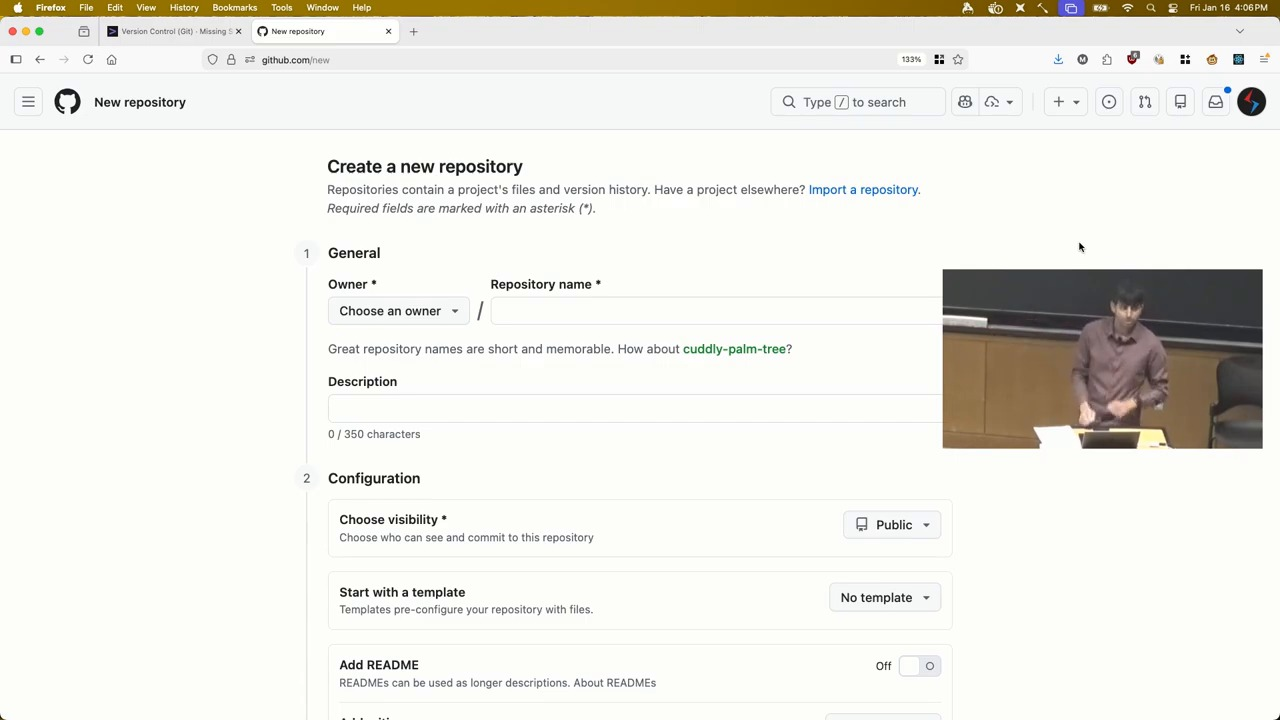
\includegraphics[width=0.92\textwidth]{figures/fig_21_github_new.jpg}
\caption{在 GitHub 上新建一个空仓库，相当于对方执行了一次 git init\vtag}
\end{figure}
\srcnote{01:01:00--01:01:15}
\end{minipage}


讲者说，到目前为止讲的是自己用 Git；Git 真正强大的地方之一是可以把本地仓库连接到某个远程仓库（remote），把修改推送过去，别人也可以向远程仓库推送修改，你再拉取到本地。他在 GitHub 上新建了一个仓库，可以是空的，设成私有。这就像“另一个人”：GitHub 只是做了一次 \texttt{git init}，没有任何历史；而他本地的仓库有一堆历史。现在把它们连起来：用 \texttt{git remote add origin} 加上地址告诉 Git 有这样一个远程仓库，名字叫 origin。

\noindent\begin{minipage}{\textwidth}
\begin{figure}[H]
\centering
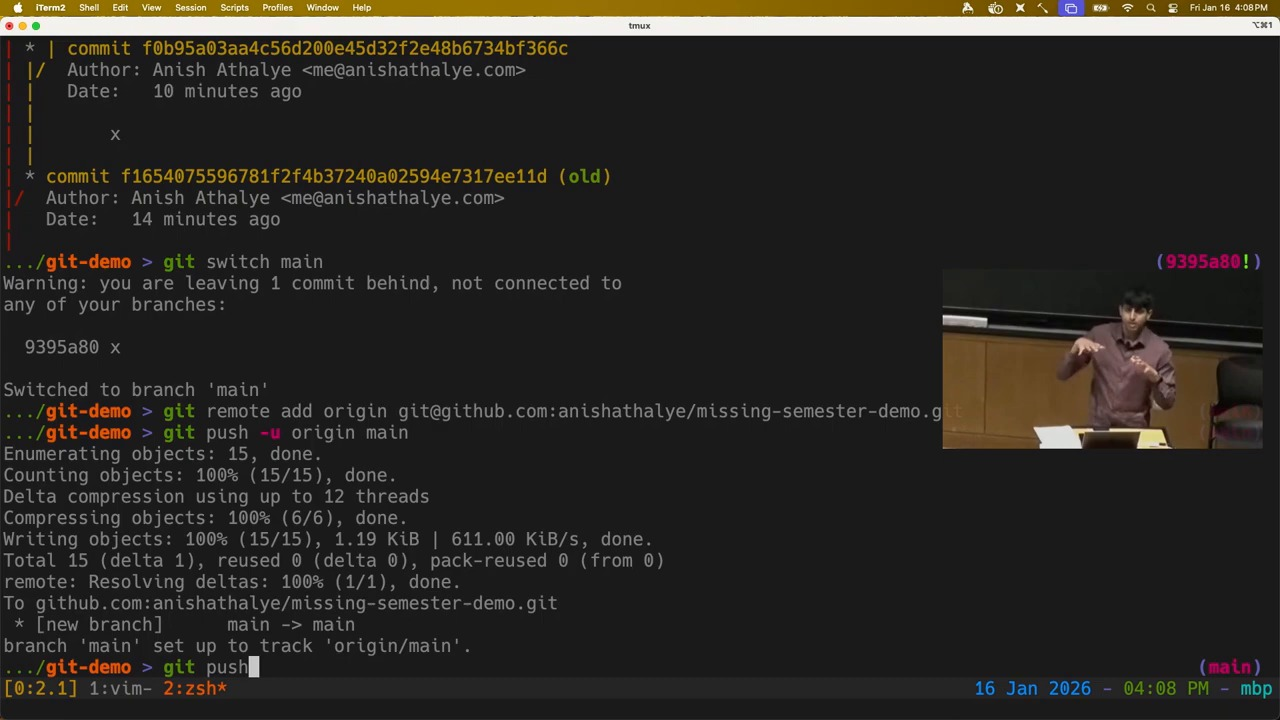
\includegraphics[width=0.92\textwidth]{figures/fig_22_push.jpg}
\caption{git push -u origin main 把本地 main 及其全部历史推送到远程\vtag}
\end{figure}
\srcnote{01:02:30--01:02:45}
\end{minipage}


然后就可以向远程仓库收发数据。\texttt{git push} 把本地修改发送到远程：\texttt{git push -u origin main} 把本地 main 分支的内容推送到远程 origin，如果远程没有 main 分支就创建一个，让它与本地 main 一致；\texttt{-u} 让本地 main 成为跟踪分支，以后本地提交后，Git 会告诉你领先远程多少，直接 \texttt{git push} 就能推送。刷新 GitHub 页面，就能看到 \texttt{nato.txt} 及其最新内容。

有同学问：推送 main 时，是只包含 main 指向的那个提交，还是整个历史？讲者说是后者：分享时总是包含通向那一点的全部历史。Git 有一些特殊命令可以截断，只接收部分历史，但那相当高级，不常用。

\subsection{克隆、拉取与获取}

\noindent\begin{minipage}{\textwidth}
\begin{figure}[H]
\centering
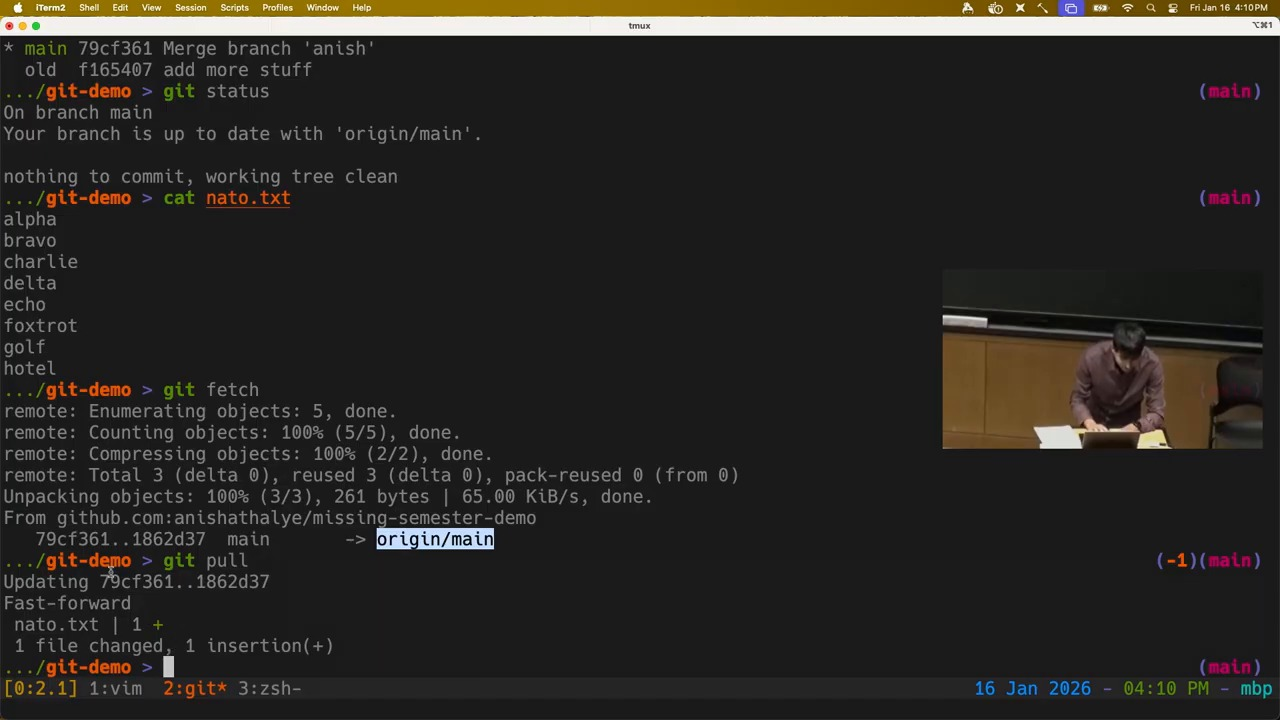
\includegraphics[width=0.92\textwidth]{figures/fig_23_fetch_pull.jpg}
\caption{在另一个副本里推送修改后，原仓库先 git fetch 再 git pull 得到更新\vtag}
\end{figure}
\srcnote{01:04:30--01:04:45}
\end{minipage}


为了演示协作，讲者假装自己是另一个人（当然是在同一台电脑上）：到桌面文件夹，用 \texttt{git clone} 克隆这个仓库，它从已有的远程仓库得到一份本地副本；进去快速加了些内容，提交并推送。回到原来的窗口，\texttt{git status}、\texttt{cat nato.txt} 都没有变化，因为还没有从远程拉取。这里有两个密切相关的命令：\texttt{git fetch} 从远程接收数据，但不改变任何本地引用；\texttt{git pull} 则会真正更新本地引用（相当于 fetch 之后再合并）。拉取之后，就看到了另一个人的修改。

讲者总结，这就是 Git 协作的方式：大家各自持有这个历史的不同切片，相互分享对历史的修改或更新，从而以非常干净的方式实现协作。Jon 在台下提醒他展示 GitHub 上的提交历史，讲者说 GitHub 是一个相当成熟的产品，其中一个好功能就是可视化提交历史。

\begin{lstlisting}[language=bash]
git remote add origin git@github.com:USER/REPO.git
git push -u origin main
git clone git@github.com:USER/REPO.git
git fetch
git pull
\end{lstlisting}

\begin{importantbox}{远程仓库也是引用}
讲义作者补充：fetch 下来的远程分支以 \texttt{origin/main} 这样的远程跟踪引用保存在本地；\texttt{git fetch} 只更新这些引用和对象存储，\texttt{git pull} 再把 \texttt{origin/main} 合并（或变基）到当前分支。用 \texttt{git log -{}-all -{}-graph} 可以同时看到本地分支和远程跟踪分支的位置。
\end{importantbox}

\subsection{差异是计算出来的}

\noindent\begin{minipage}{\textwidth}
\begin{figure}[H]
\centering
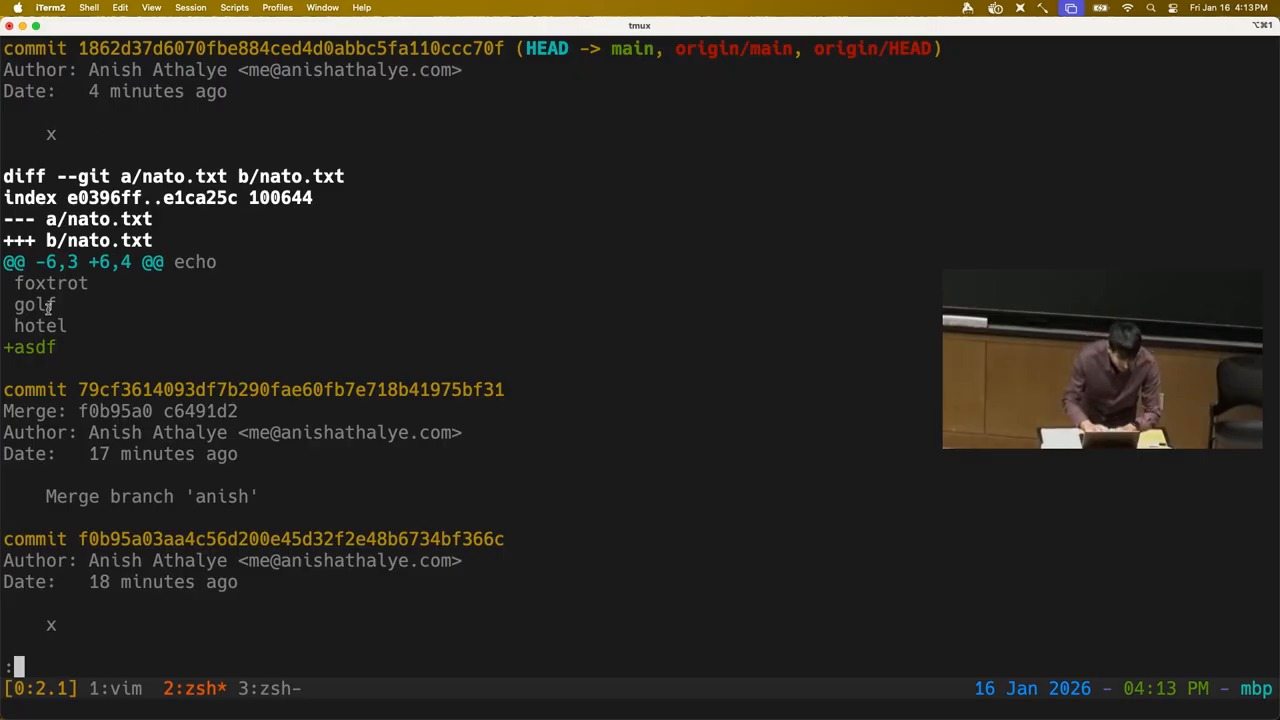
\includegraphics[width=0.92\textwidth]{figures/fig_24_diff.jpg}
\caption{git diff 计算两个快照之间的差异，显示新增了 asdf 一行\vtag}
\end{figure}
\srcnote{01:08:00--01:08:15}
\end{minipage}


讲者最后讲了差异（diff）。提交里存的不是“改了什么”，而只是“这是新的状态”，即一个快照；但查看改了什么非常方便，好在它可以计算出来：可以问 Git 这个快照和那个快照有什么区别，它会漂亮地显示出来。比如 \texttt{git log} 看最近两个提交，再对某个提交做 \texttt{git diff}，输出显示这里新增了一行 asdf。还有一个方便的命令 \texttt{git log -p}，在 log 中为每个提交内联显示差异，可以往下滚动，看到添加 asdf 的最新提交、添加 alpha 的提交、添加 hotel 的提交等等。

讲者说，Git 的界面也叫“瓷器”（porcelain），即建立在核心数据模型之上的高层命令，相当复杂，即使讲两个小时也讲不完，讲义里有更多内容和学习资源。他最后提醒大家：下周一放假，下周二再见。

\begin{practicebox}{练习}
讲义作者整理：克隆课程网站的仓库，用 \texttt{git log -{}-all -{}-graph -{}-decorate} 可视化历史；用 \texttt{git blame} 找出某一行最后是谁改的，再用 \texttt{git show} 查看那次提交；故意在两个分支上修改同一行并合并，练习解决合并冲突；最后用 \texttt{git reflog} 找回一个删除了分支的提交。
\end{practicebox}

\section{总结}

\begin{itemize}
\item 版本控制系统记录快照历史、附带元数据，支持并行开发与协作，并能回答“谁、何时、为何修改”等问题。
\item Git 的界面是有漏洞的抽象，自底向上理解数据模型才能真正用好它。
\item 文件是 blob，目录是 tree，提交指向一个顶层 tree 和若干父提交，历史是不可变的有向无环图。
\item 对象按 SHA-1 哈希进行内容寻址；引用是可变的人类可读名字，分支就是指向提交的指针；仓库就是对象加引用。
\item 暂存区让你精确决定下一个快照包含什么。
\item 常用命令：\texttt{init}、\texttt{status}、\texttt{add}、\texttt{commit}、\texttt{log}、\texttt{cat-file}、\texttt{branch}、\texttt{switch}、\texttt{merge}、\texttt{checkout}、\texttt{reflog}、\texttt{remote}、\texttt{push}、\texttt{clone}、\texttt{fetch}、\texttt{pull}、\texttt{diff}。
\end{itemize}

\begin{practicebox}{自测}
\begin{enumerate}
\item 为什么说 Git 的历史不可变，而分支可变？\texttt{git commit} 实际修改了哪些数据结构？
\item 合并提交与普通提交在数据结构上有何区别？
\item 两个内容完全相同的文件在对象存储中会存几份？为什么？
\item \texttt{git fetch} 与 \texttt{git pull} 有什么区别？
\item 进入分离 HEAD 状态后做了一个提交，怎样保住它？
\end{enumerate}
\end{practicebox}

\end{document}
